\section*{Avertissement}\label{avertissement}
\addcontentsline{toc}{section}{Avertissement}

L'African School of Economics n'entend donner ni approbation, ni
improbation aux opinions émises dans ce mémoire. Ces opinions doivent
être considérées comme propres à son auteur.

\section*{Approbation}\label{approbation}
\addcontentsline{toc}{section}{Approbation}

Nous certifions que le présent mémoire a été réalisé par son auteur. Sa
rédaction est achevée et il a été soutenu devant un jury.\\
Abomey-Calavi, le\\

\begin{longtable}[]{@{}c@{}}
\toprule\noalign{}
\endhead
\bottomrule\noalign{}
\endlastfoot
\emph{Présiden t du jury} \\
 \\
\end{longtable}

\section*{Dédicaces}\label{duxe9dicaces}
\addcontentsline{toc}{section}{Dédicaces}

{À mes frères.}

\section*{Remerciements}\label{remerciements}
\addcontentsline{toc}{section}{Remerciements}

Ce travail n'aurait pas été possible sans l'aide et la contribution de
certaine personne. Je tiens avant tout à remercier :

\begin{itemize}
\item
  le professeur Léonard WANTCHEKON, Président fondateur d'African School
  of Economics ;\\
\item
  le Dr Placide da CRUZ, Doyen des études du premier cycle d'African
  School of Economics ;\\
\item
  le Dr Maurice COMLAN, Enseignant à l'ENEAM, mon Maitre de mémoire ;\\
\item
  M. Amiel SOSSA, mon Maitre de stage, pour sa patience, sa
  disponibilité et surtout ses judicieux conseils, qui ont contribué à
  alimenter ma réflexion ;\\
\item
  Amos Sourou LEGBA, mon college de stage, camarade de promation et
  avant tout un ami très cher ;\\
\item
  tous les stagières et étudiant de LESCAL ;\\
\item
  tous mes camades de promotion ;\\
\item
  toutes ma famille pour leurs encouragement ;\\
\item
  toutes les personnes qui directement ou indirectement ont contribu à
  la russite de ce travail.\\
\end{itemize}

Merci pour vos différents contribution qui ont permis la réalisation de
ce mémoire.

\textbf{SIGLES ET ACRONYMES}

\begin{longtable}[]{@{}lll@{}}
\toprule\noalign{}
\endhead
\bottomrule\noalign{}
\endlastfoot
\textbf{LESCAL} & : & Laboratoire d'Etudes Statistique et de Conception
d'Applications \\
& & et de Logiciels ; \\
\textbf{MA} & : & Moving Average (moyenne mobile); \\
\textbf{MMa} & : & Moyenne Mobile Arithmetique ; \\
\textbf{MME} & : & Moyenne Mobile Exponentielle ; \\
\textbf{MACD} & : & Moyenne Average Convergence Divergence (Moyenne
Mobile \\
& & Convergence Divergence); \\
\textbf{BRVM} & : & Bourse Régionale des Valeurs Mobilières ; \\
\textbf{"BRVM-Agri"} & : & BRVM-Agriculture ; \\
\textbf{AUDUSD} & : & La paire de devises AUD/USD représente \\
& & le Dollar Australien (AUD) coté par rapport au Dollar Américain
(USD) ; \\
\textbf{EURUSD} & : & La paire de devises EUR/USD représente \\
& & l'Euro (EUR) coté par rapport au Dollar Américain (USD) ; \\
\textbf{GBPUSD} & : & La paire de devises GBP/USD représente \\
& & la Livre Sterling (GBP) cotée par rapport au Dollar Américain (USD)
; \\
\textbf{BRVUSDJPY} & : & La paire de devises USD/JPY représente \\
& & le Dollar Américain (USD) coté par rapport au Yen Japonais (JPY)
; \\
\textbf{XAUUSD} & : & La paire de devises XAU/USD représente \\
& & le prix de l'Or (XAU) coté par rapport au Dollar Américain (USD)
; \\
\textbf{USDCAD} & : & La paire de devises USD/CAD représente \\
& & le Dollar Américain (USD) coté par rapport au Dollar Canadien (CAD)
; \\
\end{longtable}

\section*{Résumé}\label{ruxe9sumuxe9}
\addcontentsline{toc}{section}{Résumé}

Dans le présente étude nous comparons la stratégie de trading basée sur
les Moyennes Mobile avec celle combinant l'Oscillateur Stochastique et
la Moyenne Mobile Convergence Divergence, dans le but d'évaluer leur
performance respective sur les indices BRVM-Agriculture et
BRVM-Services-Publics. L'étude a été réalisée en utilisant les données
historiques des cours des indices. Pour appliquer les stratégies, nous
avons d'abord déterminé notre profil d'investisseur, puis élaboré des
critères permettant de valider les paramètres spécifiques à chaque
stratégie, en fonction de notre profil d'investisseur. Les résultats de
cette étude ont montré que la stratégie la plus performante pour
l'indice BRVM-Agriculture est la stratégie des Moyennes Mobile, tandis
que pour l'indice BRVM-Services-Publics, la stratégie combinée de
l'Oscillateur Stochastique et de la Moyenne Mobile Convergence
Divergence s'est avérée être la plus performante. Contrairement aux
études antérieures où les stratégies de trading sont appliquées
directement avec certains paramètres, cette étude met l'accent sur la
validation des paramètres des stratégies de trading en fonction du
profil d'investisseur. Ainsi, tout investisseur sur la Bourse Régionale
des Valeurs Mobilières, notamment sur les indices BRVM-Agriculture et
BRVM-Services-Publics, possédant le profil d'investisseur spécifié dans
ce document, peut exploiter les résultats de cette étude dans sa
stratégie d'investissement. Une des limites de cette étude est qu'elle
se limite à deux indices de la Bourse Régionale des Valeurs Mobilières.

\ul{Mots clés} : BRVM , strategies de trading

\section*{Abstract}\label{abstract}
\addcontentsline{toc}{section}{Abstract}

In the context of this research, we compare the trading strategy based
on moving averages with that combining the Stochastic Oscillator and the
Moving Average Convergence Divergence, in order to assess their
performance respectively on the BRVM-Agriculture and
BRVM-Services-Publics indices. The study was carried out using
historical index price data. For each strategy, we first determined our
investor profile, then developed criteria to validate the parameters
specific to each strategy, depending on our investor profile. The
results of this study showed that the most efficient method for the
BRVM-Agriculture index is the Moving Averages strategy, while for the
BRVM-Services-Publics index, the combined strategy of the Stochastic
Oscillator and Moving Average Convergence Divergence proved to be the
best performer. Unlike previous studies where trading strategies are
applied directly with certain parameters, this study emphasizes the
validation parameters of trading strategies according to the investor
profile. Thus, any investor on the Regional Stock Exchange, in
particular on the BRVM-Agriculture and BRVM-Services-Publics indices,
with the profile investor specified in this document, may exploit the
results of this study in its investment strategy. One of the limitations
of this study is that it is limited to two stock market indices Regional
Securities.

\ul{Keywords} : BRVM , trading strategy

\section*{Introduction}\label{introduction}
\addcontentsline{toc}{section}{Introduction}

{ L'analyse technique est une méthode d'analyse utilisée en finance et
en trading pour évaluer et prévoir les mouvements futurs des prix des
actifs financiers, tels que les actions, les devises, les matières
premières, etc. Elle est largement appliquée sur les marchés financiers
depuis des décennies par les traders pour profiter du comportement
observé sur les marchés financiers. Cette approche ce base
fondamentalement sur l'étude des données historiques des cours et
volumes de ces actifs afin d'identifier des tendances, des modèles
récurrents et des signaux d'achat ou de vente. L'analyse technique
propose plusieurs méthodes pour étudier les données de marchés et
identifier les tendances et les opportunités de trading. Certains des
plus utilisés par les investisseur et les traders sont : l'analyse des
tendances, l'analyse des indicateurs technique, l'analyse des supports
et des résistances, et l'analyse des méthodes de chandeliers. Cependant
les techniques d'analyse technique ne performe pas tous sur tous les
marchés financier. Pour un investisseur soucieux de son capitale, il est
important de connaître quelle méthode choisir en fonction de sur un
marché financier spécifique. Il existe dans le monde plusieurs marchés
financier dont la Bourse régionale des valeurs Mobilières qui est une
Institution Financière Spécialisé Communautaire chargé des transactions
qui portent sur les valeurs mobilières. Sur la BRVM la actions côté sont
regroupées en sept secteurs que sont: le Secteur Industrie, le Secteur
Services Publics, le Secteur Finance, le Secteur Transport, le Secteur
Agriculture, le Secteur Distribution et le Secteur Autres. Le secteurs
Agriculture représente l'ensembles des entreprises Agriculture côté à
Bourse Régionale des Valeurs Mobile; comme PALM Côte d'Ivoire et
SUCRIVOIRE Côte D'Ivoire. Quant au Secteurs Services Publics, il
représente l'ensemble des entreprises de services publics côté à la
BRVM, principalement des entreprises de distribution télécommunication
comme SONATEL Sénégal, et les entreprises de distribution électrique
comme CIE Côte D'Ivoire. Pour chaque secteur, la BRVM dispose des
indices qui mesure la performance des entreprises côtes dans le secteur
spécifique. Ainsi la BRVM-Agriculture est un indice qui mesure
l'évolution des cours des actions des secteurs agricole et la
BRVM-Services-Publics qui représentant l'évolution du cours des actions
des entreprises de Services Publics côté à la BRVM. Pour tout
investisseur désireux d'investir et de profiter de l'évolution de
l'Agriculture dans l'espace UEMOA ou des Services Publics il est
important de connaître quelle stratégie de trading ou quel indicateur
technique utilisé afin de comprendre et de profiter de l'évolution des
cours des actifs sur le marché. Le présent document s'intéresse à une
comparaison de deux stratégies de trading sur l'indice BRVM-Agriculture,
et l'indice BRVM-Services-Publics ; la stratégie des Moyennes Mobile, et
la stratégie combinée de l'Oscillateur Stochastique et de la Moyenne
Mobile Convergence Divergence, ainsi qu'aux meilleurs paramètres de
chaque stratégie. Ce document est subdiviser en trois partie: la
première chapitres. Dans le premiers chapitres intitulé cadre
institutionnel et observation du stage, nous allons présenter le cadre
institutionnel qu'est LESCAL puis dans le chapitre 2 nous allons parler
de la méthodologie puis enfin dans le chapitre trois nous allons
appliquer les stratégie de trading sur les différents données et
présenter les résultats. }

\section{CADRE INSTITUTIONNEL ET OBSERVATION DU
STAGE}\label{cadre-institutionnel-et-observation-du-stage}

\subsection{Présentation du LESCAL}\label{pruxe9sentation-du-lescal}

\subsubsection{\texorpdfstring{ Historique, missions, objectifs et
activités du
LESCAL}{ Historique, missions, objectifs et activités du LESCAL}}\label{historique-missions-objectifs-et-activituxe9s-du-lescal}

\paragraph{Historique du LESCAL}\label{historique-du-lescal}

Le Laboratoire d'Etudes Statistiques et de Conception d'Applications et
logiciels, LESCAL est le fruit de la collaboration entre statisticiens
et informaticiens qui l'ont créé en Juillet 2017. LESCAL autrefois
dénommé LES (Laboratoire d'Etudes Statistiques) était une initiative
dont l'objet était d'apporter un appui aux étudiants statisticiens et
non statisticiens pour le traitement des données (analyses statistiques
avancées, différentes régressions, méthodes de prévision) dans le cadre
de la rédaction de leur mémoire de fin de formation (licence, master,
doctorat).

Deux années plus tard (2019), certains membres de l'équipe, aspirant aux
nouvelles technologies ont étendu les domaines d'intervention du LESCAL
au secteur du numérique d'où le suffixe « CAL » (Conception
d'Applications et Logiciels), ce qui engendra LESCAL. A nos jours le
laboratoire intervient dans les divers domaines que sont : le traitement
et l'analyse des données statistiques, le génie logiciel et
l'intelligence artificielle.

\paragraph{Missions et activités du
LESCAL}\label{missions-et-activituxe9s-du-lescal}

LESCAL intervient sur deux principaux volets : le génie logiciel et
l'intelligence artificielle. Conformément au premier, LESCAL répond aux
besoins des entreprises, des chercheurs, des professionnels, des
particuliers en termes de solutions informatiques destinées à divers
usages: Business analytics (analyse commerciale), comptabilité,
facturation, site internet, application mobile, etc. D'autre part, il
conçoit des solutions d'intelligence artificielle dans les domaines :
reconnaissance visuelle (computer vision), compréhension du langage
humain (Natural Language Processing). Par ailleurs à travers son vaste
programme LESCAL ACADEMY, il offre aux étudiants, aux professionnels et
au personnel des entreprises une gamme variée de formations dans le
domaine du numérique et de la science des données et contribue à
l'insertion professionnelle des jeunes par des programmes de stage.

\paragraph{Objectifs de LESCAL}\label{objectifs-de-lescal}

LESCAL a pour objectif de:

\begin{itemize}
\item
  promouvoir la statistique dans tous les secteurs d'activité ;\\
\item
  promouvoir les métiers du numérique ;\\
\item
  aider à la gestion statistique informatisée pour une bonne prise de
  décision;\\
\item
  former des cadres compétents et de qualité pour la relève.
\end{itemize}

\subsubsection{\texorpdfstring{Organisation, fonctionnement,
environnement et localisation\\
géographique du
LESCAL}{Organisation, fonctionnement, environnement et localisation géographique du LESCAL}}\label{organisation-fonctionnement-environnement-et-localisation-guxe9ographique-du-lescal}

\paragraph{Localisation et
Organisation}\label{localisation-et-organisation}

Situation géographique de la structure\\
Siège : Bénin, Abomey-Calavi\\
Téléphone : (+229) 97 67 57 68\\
Email: lescal@gmail.com et lescal@lescal-soc.com\\
L.E.S.C.A.L. est organisé en Unités de Formation et de Recherche (UFR),
ce qui correspond au modèle universitaire, celui-ci se voulant digne des
recherches contribuant aux innovations technologiques, voulant
accompagner les jeunes étudiants des filières du numérique. Les Unités
de Formation et de Recherche dont il est constitué sont les suivantes :

\begin{itemize}
\item
  UFR Datasciences / Intelligence Artificielle
\item
  UFR Ingénierie logiciels desktops
\item
  UFR ingénierie applications mobiles
\item
  UFR ingénierie du web / développement web
\end{itemize}

Ainsi les étudiants sollicitant un stage ou une formation sont alors
insérés dans l'une des Unités de Formation et de Recherche selon leurs
talents et leurs aspirations professionnelles. Le Laboratoire d'Etudes
Statistiques et de Conception d'Applications et Logiciels s'organise
pour créer une structure professionnelle et de façon à pouvoir mener à
bien les objectifs de l'institution. L'organigramme du laboratoire se
présente comme suit :

\begin{figure}
\centering
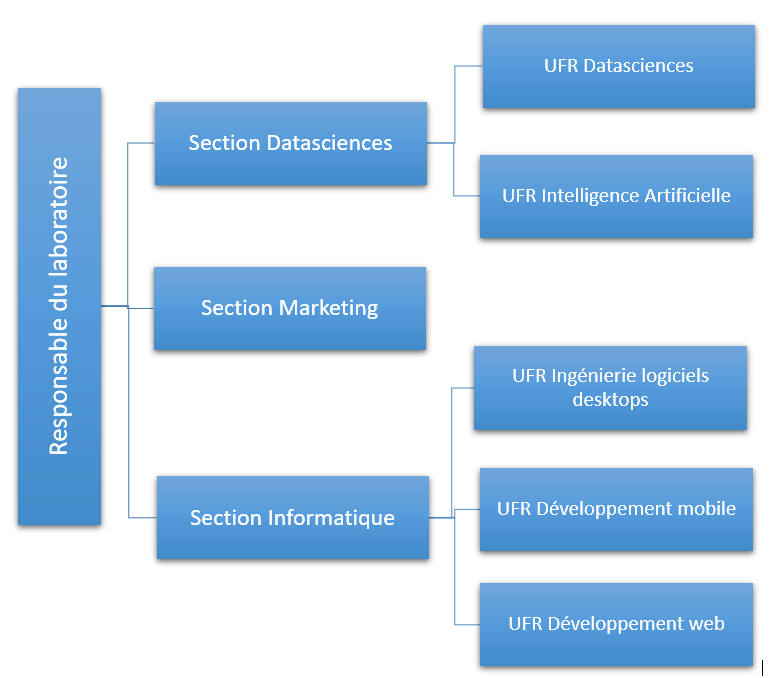
\includegraphics{img/orga.png}
\caption{Organigramme de LESCAL}
\end{figure}

\paragraph{Fonctionnement}\label{fonctionnement}

LESCAL étant un laboratoire de recherche qui vise à contribuer aux
innovations technologique, il est subdivisé en quatre grandes Unités de
Formation et de Recherche (Data sciences / Intelligence Artificielle,
ingénierie logiciels desktops, ingénierie applications mobiles,
ingénierie du web). Le responsable du laboratoire définit les rôles et
attributions de chaque UFR ; chaque UFR étant dirigée par un sous
responsable qui se charge de coordonner les travaux des membres dans
l'atteinte des objectifs généraux du laboratoire.

\subsubsection{Environnement micro et
macro}\label{environnement-micro-et-macro}

\paragraph{Le micro-environnement}\label{le-micro-environnement}

Le microenvironnement de LESCAL est l'ensemble de tous les éléments qui
exercent une influence sur les activités du laboratoire, il s'agit de la
concurrence, la clientèle, les fournisseurs.

\paragraph{La Concurrence}\label{la-concurrence}

Le laboratoire L.E.S.C.A.L vit dans un environnement fortement
concurrentiel compte tenu de la nature de ses services. Ses concurrents
sont l'ensemble des entreprises dont les services sont directement ou
indirectement substituables aux siens. L'analyse de la concurrence étant
d'une importance fondamentale pour toute entreprise quelle que soit sa
taille, doit lui permettre d'innover, de perfectionner ses produits afin
de satisfaire au maximum ses clients et se faire attribuer la plus
grande part de marché.

\paragraph{La clientèle}\label{la-clientuxe8le}

La clientèle est constiltuée des consommateurs actuels et potentiels qui
s'intéressent à l'offre du laboratoire. Il s'agit des acheteurs ou
consommateurs des services. Elle regroupe l'ensemble des opérateurs
réels et potentiels des services du laboratoire. En effet, la clientèle
étant un élément principal de fonds de commerce, toute décision
commerciale doit tenir compte de ses désirs et attentes.

\paragraph{Les fournisseurs}\label{les-fournisseurs}

Il s'agit des entreprises qui fournissent à au laboratoire L.E.S.C.A.L
tout ce dont elle a besoin pour son fonctionnement. Il s'agit des
fournisseurs d'intrants, de fournisseurs de services généraux
(fourniture d'énergies, d'eau, de communications). Ici, ils représentent
les tiers, qui peuvent être des personnes physiques ou morales qui,
approvisionnent la société en prestations diverses. Ainsi, les
fournisseurs peuvent être regroupés en deux (02) catégories :

\begin{itemize}
\item
  les prestataires de services ;
\item
  les équipementiers.
\end{itemize}

\paragraph{Le macro-environnement}\label{le-macro-environnement}

On le définit comme l'ensemble des grandes tendances du laboratoire dans
sa globalité. La caractéristique et l'évolution du macro-environnement
s'imposent au laboratoire: en aucun cas, elle n'a la possibilité
d'interagir avec. Il s'agit notamment de:

\paragraph{l'environnement politico-légal ou
réglementaire}\label{lenvironnement-politico-luxe9gal-ou-ruxe9glementaire}

Tout comme le marché béninois, l'environnement politico-légal ou
réglementaire est aujourd'hui fortement marqué par le libéralisme
économique. Au plan législatif, la loi N° 90-005 du 15 mai 1990 fixant
les conditions d'exercice des activités du commerce en République du
Bénin affirme les principes de la liberté du commerce au Bénin et
apporte les allègements substantiels aux procédures d'implantation des
entreprises commerciales étrangères. Au plan réglementaire, les nouveaux
textes simplifient les procédures d'exclusion des commerçants en rendant
plus libre le commerce au Bénin.

\paragraph{L'environnement économique et
technologique}\label{lenvironnement-uxe9conomique-et-technologique}

La définition d'un marché ne tient pas compte seulement de l'aspect
quantitatif mais aussi de l'aspect qualitatif en terme de pouvoir
d'achat des clients actuels et potentiels L'économie béninoise est
actuellement caractérisée par une diminution du pouvoir d'achat de la
population due à l'inflation dont le taux moyen est de 2,5\% en 2005.
Selon les données statistiques, une entreprise dont l'environnement
technologique doit couvrir essentiellement les nouvelles technologies
dans les domaines de l'information et de la communication et de
l'informatique appartenant aux innovations de pointe.

\paragraph{L'environnement démographique et
socioculturel}\label{lenvironnement-duxe9mographique-et-socioculturel}

Le centre évolue sur un marché à forte croissance à cause de la poussée
démographique que connaît le Bénin. Avec une superficie de 114 763 km2
et un taux de croissance de 3.25\% selon le Recensement Général de la
Population et de l'Habitat, la population du Bénin est en plein
croissance. Le rythme de la croissance démographique présente un intérêt
pour le monde des affaires car l'augmentation de la population entraîne
un accroissement de la demande des offres et donc un développement de ce
marché.

\subsection{Déroulement du stage}\label{duxe9roulement-du-stage}

\subsubsection{Entitées parcourues et tâches
exécutées}\label{entituxe9es-parcourues-et-tuxe2ches-exuxe9cutuxe9es}

{Nos quatres mois de stages au Laboratoire d'Etude Statistiques et de
Conception d'Applications et Logiciels ont été marqué par plusieurs
activités. Tous d'abord nous avons commencer par un mois d'inition au
concept des marchés financier, su trading et des stratégies de trading.
Puis nous avons suivi et réaliser des formations et des activités dans
les UFR suivant. De plus nous avons eu à enseigner des cours de
programmation Python et de programmation C. }

{Nous avons suivi une formation en computer vision en Deep Learning et
en reconnaissance du langage humain. Lors de la formation en conputer
vision nous avons écrire et entrainer des model d'IA qui permettent de
reconnaitre des bateaux.}

{En ingénierie logiciel, nous avons participer à la Conception d'une
application d'intelligence Artificielle visant à relever automatiquement
des les notes des éleves depuis une images vers un fichiers Excel. Dans
ce projet nous nous somme occuper du volet UI de l'application.
Également nous avons concu une application qui à pour rôle d'optimiser
le temps de calcul des paramètres des systèmes de distibution d'eau en
parapluie et en surpression.}

\subsubsection{Observations du stage et difficultées
rencontrées}\label{observations-du-stage-et-difficultuxe9es-rencontruxe9es}

\paragraph{Observations du stage}\label{observations-du-stage}

{À LESCAL les étudiants et les stagiaires sont très passionner par les
Datasciences, la programmation et l'Intelligence Artificielle. Ce qui
permet de faire de nouvelles connaissance et d'être entourrer des
personnes partagant des mêmes sens d'interet. Durant notre stage nous
avons été confronté à plusieurs difficulté. En effet il faut noter qu'à
LESCAL la connection Internet n'est pas toujours disponoble quand on en
a besoin. Ce qui ne permet pas de pouvoir accès à l'information en temps
voulu. Même si toute les dispositions matériels de base telles que
l'acces sans faille à l'électricité, les meubles etc... sont présentes
il faut noter que en temps de saison sèche, il manque de système de
ventillation afin de permettre un cadre aiéré en temps de chaleur. }

\paragraph{Expériences accumulées}\label{expuxe9riences-accumuluxe9es}

{Durant nos quatre mois de stage au Laboratoire d'Etude Statistique et
de Conception d'Applications et Logicils, nous avons acquet des
expériences dans le domaine de l'Intelligence Artificielle, de la
finance et surtour dans le developpement d'application Desktop et le
developpement web. De plus de part les recherches en programmation dans
le cadre de l'accomplissement de certains travaux de laboratoire, nous
avons consolider nos acquis en programmation python, notamment la
manipulation des images et des videos sous python et le web scrapping.
De même de part nous avons consolider nos acquis en programmation C.}

\section{CADRE THEORIQUE ET METHODOLOGIE DE
L'ETUDE}\label{cadre-theorique-et-methodologie-de-letude}

\subsection{Cadre théorique de
l'étude}\label{cadre-thuxe9orique-de-luxe9tude}

\subsubsection{Problématique, intérêts, objectifs et hypothèses de
l'étude}\label{probluxe9matique-intuxe9ruxeats-objectifs-et-hypothuxe8ses-de-luxe9tude}

\paragraph{Problématique et intérêt de
l'étude}\label{probluxe9matique-et-intuxe9ruxeat-de-luxe9tude}

Dans un monde de plus en plus orienté vers l'économie de la
financiarisation, le nombre d'actifs financiers augmente de façon
exponentielle, de même que le nombre d'investisseurs. En effet, en 2020,
la valeur des actifs financiers détenus par l'ensemble de la population
mondiale a augmenté de 10\%, atteignant 200 000 milliards d'euros. De
plus en plus nombreux, les investisseurs attendent des signaux propices
à l'investissement sur les marchés boursiers avant de passer à l'action.
Ce n'est qu'en apprenant l'analyse du marché du trading ou des actions
qu'un investisseur peut prendre des décisions intelligentes et, par
conséquent, des bénéfices. Parmi les analyses faites en trading, on
trouve l'analyse technique. Elle consiste principalement à analyser une
tendance ayant une représentation graphique{[}1{]}. En réalité, il
existe plusieurs méthodes de l'analyse technique permettant de prévoir
;es tendance du marché. Il existe un grand nombre de méthodes et
d'approches différentes pour analyser les mouvements des prix des actifs
financiers.

Il est donc très difficile pour les investisseurs de choisir le meilleur
indicateur technique et, par conséquent, de maximiser leurs revenus.
Cette étude s'intéresse au marché boursier de l'UEMOA qu'est la Bourse
Régionale des Valeurs Mobilières (BRVM), en particulier à l'indice
BRVM-Agriculture qui suit la performance des entreprises du secteur
agricole cotées à la Bourse Régionale des Valeurs Mobilières. Il fournit
une valeur de référence pour évaluer la performance des entreprises du
secteur agricole en Afrique de l'Ouest et à l'indice
BRVM-Services-Publics qui suit les performances des entreprises du
secteur publics. En raison du développement continu de l'agriculture et
des entreprises proposant des services publics (notamment les
entreprises des télécommunication), dans la région de l'Afrique de
l'Ouest, la BRVM-Agriculture et la BRVM-Services-Publics sont des
indices précieux pour les investisseurs désireux de profiter du
potentiel de croissance de l'agriculture et des services publics dans
cette zone géographique. Il est donc nécessaire de savoir quand les prix
sont susceptibles d'augmenter ou de diminuer et quelle et surtout
quelles stratégie utiliser pour . À cet effet, plusieurs indicateurs
techniques et algorithmes existent afin de prédire et de générer les
signaux d'achat et de vente. L'intérêt de notre étude est de trouver le
meilleur indicateur technique entre l'indicateur Moyenne Mobile, et
l'indicateur combiné de l'Oscillateur Stochastique et de la Moyenne
Mobile Convergence Divergence.

\paragraph{Objectifs de l'étude}\label{objectifs-de-luxe9tude}

L'objectif général de cet étude est de comparer la stratégies de trading
basé sur les Moyennes Mobiles à la méthode combinée de l'osciateurs
stochastiques et de la moyenne mobile convergence divergence. Il s'agira
de :

\begin{itemize}
\item
  {Appliquer la stratégie des Moyennes Mobiles sur l'indice
  BRVM-Agriculture;}
\item
  {Appliquer la méthodes combiné de l'osciateurs stochastique et de la
  Moyenne Mobile Convergence Divergence;}
\item
  {Appliquer la methode du backtesting sur les deux stratégies de
  trading}
\end{itemize}

\paragraph{Hypothèses}\label{hypothuxe8ses}

\(-H_1\){ : La méthode des Moyennes Mobiles génère plus de signal
d'achat et de ventes que le que la méthodes de l'oscillateur
stochastique combinée à la méthodes des Moyennes Mobiles. }\\
\(-H_2\){ : La méthodes de l'oscillateur stochastique combinée à la
méthodes des Moyennes Mobiles produit plus de bénéfice à l'investisseur
}\\

\subsubsection{Revue de littérature}\label{revue-de-littuxe9rature}

\paragraph{Clarifications
conceptuelles}\label{clarifications-conceptuelles}

\textbf{Marché financier}

Un marché financier est un lieu, physique ou virtuel, où les acteurs du
marché (acheteurs, vendeurs) se rencontrent pour négocier des produits
financiers. Il permet de financer l'économie, tout en permettant aux
investisseurs de placer leur épargne.

\textbf{Trading financier}

Le trading est l'activité qui consiste à spéculer sur les marchés
financiers dans le but de réaliser des profits. Elle consiste à acheter
ou à vendre différents types d'actifs financiers, tels que des actions,
des devises (Forex Trading ou Trading Forex), des matières premières et
des crypto-monnaies, entre autres. Plus l'actif est liquide, mieux
c'est.

\textbf{Actifs financiers}

Un actif financier est un titre ou un contrat, généralement
transmissible et négociable, par exemple sur un marché financier, qui
est susceptible de produire à son détenteur des revenus ou un gain en
capital, en contrepartie d'une certaine prise de risque. Pour un
particulier propriétaire d'un tel instrument, un actif financier est
considéré comme un placement et est compté dans son patrimoine. Les
instruments financiers sont généralement les obligations légales d'une
partie de transférer un actif/valeur (généralement de l'argent) à une
autre partie à une date ultérieure et sous certaines conditions. Afin de
comprendre les instruments financiers, il faut savoir qu'ils sont en
fait des actifs qui peuvent être tradés. Ces actifs peuvent être de
l'argent comptant, des droits contractuels de livrer ou de recevoir de
l'argent ou un autre type d'instrument financier ou une preuve de
propriété d'une entité économique.

\textbf{Indices boursiers}

Un indice boursier est un indicateur calculé sur la base des valeurs
d'actions et/ou d'obligations des sociétés publiques, collectées selon
un certain critère. Il peut s'agir des plus grandes entreprises d'un
pays ou d'un secteur en termes de capitalisation. L'indice boursier joue
un rôle d'indicateur de l'état du marché boursier et de l'économie des
différents secteurs ou de l'ensemble d'un pays. La croissance de
l'indice implique le développement, tandis que la récession montre les
problèmes existants.

\textbf{Portefeuille d'actifs}

Un portefeuille désigne un ensemble d'actifs financiers détenus par un
individu ou un organisme financier dans le but d'optimiser son rendement
tout en minimisant le risque. Les différents titres qui composent le
portefeuille sont choisis de manière à obtenir un rendement global qui
soit le plus élevé et le moins risqué possible.

\textbf{Le cours d'un actif financier}

Le cours d'une action correspond au montant nécessaire pour acheter une
action d'une société. Le cours d'une action n'est pas fixe. Il varie
selon les conditions du marché. Le cours augmentera probablement si la
société semble bien se porter et chutera si elle ne répond pas aux
attentes.

\textbf{Stratégie de trading}

Une stratégie de trading représente le plan d'action qu'un trader
utilise pour tous ses traders sur les marchés financiers. Elle est
essentielle pour tout investisseur, qu'il soit débutant ou
professionnel, de sorte que toute décision de trading soit informée et
en concordance avec un plan rigoureux. Les stratégies de trading créent
un ensemble de règles ou une méthodologie pour faciliter le processus de
prise des décisions de trading.

\textbf{Analyse fondamentale en finance}

L'analyse fondamentale est une méthode d'analyse basée sur l'étude des
fondamentaux économiques. Elle consiste à déterminer la valeur
intrinsèque d'un actif financier pour la comparer à sa valeur de marché.
Si la valeur intrinsèque obtenue par l'analyse fondamentale de l'actif
est inférieure à sa valeur de marché, alors l'actif est sous-valorisé. À
l'inverse, si la valeur intrinsèque est supérieure à la valeur de
marché, alors l'actif est surévalué. L'analyse fondamentale peut
s'appliquer à n'importe quel marché financier, qu'il s'agisse des
actions, des indices boursiers, des obligations, des devises ou des
matières premières. Certains investisseurs vedettes tels que Warren
Buffet en ont d'ailleurs fait le cœur de leur stratégie avec
l'investissement value.

\textbf{Analyse technique en finance}

L'analyse technique est une méthode de compréhension des marchés
financiers reposant sur l'étude des prix et des volumes, de leurs
fluctuations et des configurations qu'ils forment. Le trader et
l'investisseur « techniciens » recherchent des configurations -- ou
patterns -- susceptibles de se répéter selon une certaine probabilité.
Le technicien souhaite en effet déceler des configurations à fortes
probabilités afin d'obtenir un avantage concurrentiel décisif sur les
marchés.

\textbf{Moyenne Mobile}

La moyenne mobile, ou moyenne glissante, est un type de moyenne
statistique utilisée pour analyser des séries ordonnées de données, le
plus souvent des séries temporelles, en supprimant les fluctuations
transitoires. Elle est également utilisée dans le milieu du trading en
tant qu'indicateur de tendance.

\paragraph{Travaux antérieurs}\label{travaux-antuxe9rieurs}

\textbf{-Comparison Between Exponential Moving Average Based MACD with
Simple Moving Average Based MACD of Technical Analysis par Vyas
street,Nr. Hanuman Gali,Upali, Bazar, Decembre 2013}

{L'objectif de cette étude était de trouver la méthode des Moyennes
Mobiles Convergence Divergence qui générait le plus de profits, le
maximum de signaux et un bon rendement. Elle a été réalisée en utilisant
les prix de clôture quotidiens par an (01-04 au 31-03) sur trois années
consécutives à partir de 2010 de la CNX Nifty qui est un indice boursier
indien composé de 50 des principales capitalisations boursières du pays.
L'étude a montré que la stratégie des MACD basée sur la Moyenne Mobile
Exponentielle est la plus performante avec un revenu total de 63.61\%
contre 24.61\% générés par la méthode basée sur la Moyenne Mobile
Simple.}

\textbf{-Technology and Investment, 2010 :A Comparison of Stock Market
Efficiency of the BRIC Countries par Terence, Sam \& Elfreda}

{Cette étude a pour but de mesurer la rentabilité des stratégies de
trading basées sur des indicateurs techniques associés à la Moyenne
Mobile Simple (SMA), l'Indice de Force Relative (RSI), la Moyenne Mobile
Convergence Divergence (MACD) et le Momentum (MOM) sur les marchés
boursiers du Brésil, de l'Inde, de la Russie et de la Chine. Cette étude
a montré que c'est la méthode des Moyennes Mobiles Simple de période 10
qui générait le plus de revenu, soit 60,58\% pour l'indice Russe RST. Il
ressort également de cette étude que la Moyenne Mobile de période 50 est
le meilleur indicateur pour les indices BSE Sensex (Inde) et SZES
(Chine) Composite. Enfin, la MACD (12,26,14) était le meilleur
indicateur pour l'indice Chinois SSEA.}

\textbf{- Performance Comparison of Three Automated Trading Systems
(MACD, PIVOT and SMA) by Means of the d-Backtest PS Implementation par
D. Th. Vezeris and C. J. Schinas}

{Dans cette etude, Vezeris et Schinas cherche à évaluer la performance
des stratégie de trading algorithmique, basé sur la MACD(MOyenne Mobile
Convergence Divergence), SMA (moyenne mobile arithmétique) et le PIVOT
points (croisement des prix). L'étude a été réalisé en utilisant les
prix de clôture des devises : AUDUSD, EURUSD, GBPUSD, USDCAD,USDJPY,
XAUUSD entre le 28/2/2016 et le 27/8/2017. En termes de rentabilité, le
système de trading MACD adaptatif a été le plus efficace, suivi du
système commercial PIVOT et le SMA a été classé comme le système
commercial le moins rentable.}

\textbf{- The profitability of MACD and RSI trading rules in the
Australian stock market par Safwan Mohd Nor et Guneratne
Wickremasinghe.}

{ Cette étude examine la rentabilité entre deux stratégie de trading :
la convergence de la moyenne mobile Divergence (MACD) et l'indice de
force relative (RSI) í sur le marché boursier australien. Elle a été
réaliser en utilisant les données de 1996 à 2014 sur l'Australian All
Ordinaries Index. D'après cette étude, la stratégie de la MACD et le RSI
peuvent générer des profils sur le marché financier Australien. Cette
étude suggèrent que le marché boursier l'Australie n'est pas efficace
dans la forme faible. Les résultats de cette recherche appuient l'idée
de constamment réviser les stratégies de trading existantes et optimiser
les paramètres des règles de négociation afin d'exploiter inefficacité
du marché.}

\subsection{Méthodologie de la
recherche}\label{muxe9thodologie-de-la-recherche}

\subsubsection{\texorpdfstring{ Présentation des données
}{ Présentation des données }}\label{pruxe9sentation-des-donnuxe9es}

\paragraph{Données brute}\label{donnuxe9es-brute}

{ Les données que nous utilisont dans cette étude proviennent du site
web investing.com. Il s'agit des données de cours journalière des
indices : }

\begin{itemize}
\item
  BRVM-Agriculture

  \hypertarget{tab:multirow}{}
  \begin{longtable}[]{@{}llllll@{}}
  \caption{Présentation des données de la
  BRVM-Agriculture}\tabularnewline
  \toprule\noalign{}
  Date & Dernier & Ouv & Plus Haut & Plus Bas & Variation\% \\
  \midrule\noalign{}
  \endfirsthead
  \toprule\noalign{}
  Date & Dernier & Ouv & Plus Haut & Plus Bas & Variation\% \\
  \midrule\noalign{}
  \endhead
  \bottomrule\noalign{}
  \endlastfoot
  29/11/2021 & 247,95 & 244,32 & 248,97 & 244,32 & 1,49\% \\
  30/11/2021 & 248,36 & 247,95 & 248,43 & 247,95 & 0,17\% \\
  01/12/2021 & 249,12 & 248,36 & 250,45 & 248,36 & 0,31\% \\
  02/12/2021 & 250,05 & 249,12 & 251,09 & 250,05 & 0,37\% \\
  03/12/2021 & 243,92 & 250,05 & 250,05 & 243,92 & -2,45\% \\
  ... & ... & ... & ... & ... & ... \\
  09/05/2023 & 260,09 & 263,37 & 263,37 & 260,09 & -1,25\% \\
  10/05/2023 & 253,34 & 260,09 & 263,07 & 247,71 & -2,60\% \\
  11/05/2023 & 251,77 & 253,34 & 254,20 & 243,82 & -0,62\% \\
  12/05/2023 & 249,87 & 251,77 & 253,49 & 243,25 & -0,75\% \\
  15/05/2023 & 248,05 & 249,87 & 250,58 & 243,85 & -0,73\% \\
  \end{longtable}
\item
  BRVM-Services publics

  \hypertarget{tab:multirow}{}
  \begin{longtable}[]{@{}llllll@{}}
  \caption{Présentation des données de la BRVM-Service
  Public}\tabularnewline
  \toprule\noalign{}
  Date & Dernier & Ouv & Plus Haut & Plus Bas & Variation\% \\
  \midrule\noalign{}
  \endfirsthead
  \toprule\noalign{}
  Date & Dernier & Ouv & Plus Haut & Plus Bas & Variation\% \\
  \midrule\noalign{}
  \endhead
  \bottomrule\noalign{}
  \endlastfoot
  26/11/2021 & 440,30 & 440,62 & 445,25 & 440,30 & -0,07\% \\
  29/11/2021 & 442,39 & 440,30 & 449,47 & 440,30 & 0,47\% \\
  30/11/2021 & 450,26 & 442,39 & 450,36 & 442,39 & 1,78\% \\
  01/12/2021 & 449,67 & 450,26 & 450,26 & 449,67 & -0,13\% \\
  02/12/2021 & 449,50 & 449,67 & 450,09 & 449,50 & -0,04\% \\
  ... & ... & ... & ... & ... & ... \\
  09/05/2023 & 481,66 & 479,45 & 481,76 & 478,08 & 0,46\% \\
  10/05/2023 & 482,27 & 481,66 & 492,36 & 479,30 & 0,13\% \\
  11/05/2023 & 486,77 & 482,27 & 486,77 & 480,22 & 0,93\% \\
  12/05/2023 & 489,95 & 486,77 & 490,69 & 483,95 & 0,65\% \\
  15/05/2023 & 468,96 & 489,95 & 489,95 & 459,94 & -4,28\% \\
  \end{longtable}
\end{itemize}

\paragraph{Données pré-traité}\label{donnuxe9es-pruxe9-traituxe9}

\textbf{Stratégie des Moyennes Mobiles.}

\hypertarget{tab:multirow}{}
\begin{longtable}[]{@{}llllll@{}}
\caption{Données Pré-traités pour la stratégie des Moyennes Mobiles pour
l'indice BRVM-Agriculture}\tabularnewline
\toprule\noalign{}
Date & Dernier & Ouv & Variation & MA26 & MA61 \\
\midrule\noalign{}
\endfirsthead
\toprule\noalign{}
Date & Dernier & Ouv & Variation & MA26 & MA61 \\
\midrule\noalign{}
\endhead
\bottomrule\noalign{}
\endlastfoot
03/09/2020 & 65,30 & 67,55 & -3,33\% & 60,16 & 61,63 \\
04/09/2020 & 65,42 & 65,30 & 0,18\% & 60,50 & 61,63 \\
07/09/2020 & 65,35 & 65,42 & -0,11\% & 60,91 & 61,65 \\
08/09/2020 & 66,64 & 65,35 & 1,97\% & 61,37 & 61,69 \\
09/09/2020 & 66,83 & 66,64 & 0,29\% & 61,84 & 61,75 \\
... & ... & ... & ... & ... & ... \\
09/05/2023 & 260,09 & 263,37 & -1,25\% & 275,57 & 284,27 \\
10/05/2023 & 253,34 & 260,09 & -2,60\% & 274,15 & 283,54 \\
11/05/2023 & 251,77 & 253,34 & -0,62\% & 272,80 & 282,78 \\
12/05/2023 & 249,87 & 251,77 & -0,75\% & 271,32 & 281,95 \\
15/05/2023 & 248,05 & 249,87 & -0,73\% & 269,76 & 281,12 \\
\end{longtable}

\hypertarget{tab:multirow}{}
\begin{longtable}[]{@{}llllll@{}}
\caption{Données Pré-traités pour la stratégie des Moyennes Mobiles
pour\\
l'indice BRVM-Service Public}\tabularnewline
\toprule\noalign{}
Date & Dernier & Ouv & Variation & MA48 & MA98 \\
\midrule\noalign{}
\endfirsthead
\toprule\noalign{}
Date & Dernier & Ouv & Variation & MA48 & MA98 \\
\midrule\noalign{}
\endhead
\bottomrule\noalign{}
\endlastfoot
03/11/2020 & 355,67 & 370,36 & -3,97\% & 360.05 & 373.16 \\
04/11/2020 & 357,55 & 355,67 & 0,53\% & 359.51 & 372.76 \\
05/11/2020 & 361,29 & 357,55 & 1,05\% & 359.04 & 372.38 \\
06/11/2020 & 358,76 & 361,29 & -0,70\% & 358.61 & 372.01 \\
09/11/2020 & 357,66 & 358,76 & -0,31\% & 358.16 & 371.64 \\
... & ... & ... & ... & ... & ... \\
09/05/2023 & 481,66 & 479,45 & 0,46\% & 487.29 & 486.53 \\
10/05/2023 & 482,27 & 481,66 & 0,13\% & 487.08 & 486.74 \\
11/05/2023 & 486,77 & 482,27 & 0,93\% & 486.88 & 487.00 \\
12/05/2023 & 489,95 & 486,77 & 0,65\% & 486.70 & 487.29 \\
15/05/2023 & 468,96 & 489,95 & -4,28\% & 485.98 & 487.37 \\
\end{longtable}

\textbf{Stratégie Combiné de l'Oscillateur Stochastique et de}\\
\textbf{la moyenne Mobile Convergence Divergence.}

\hypertarget{tab:multirow}{}
\begin{longtable}[]{@{}llllllllll@{}}
\caption{Données Pré-traités pour la stratégie Combiné de l'Oscillateur
Stochastique et de la moyenne Mobile Convergence Divergence pour
l'indice BRVM-Agriculture}\tabularnewline
\toprule\noalign{}
\endfirsthead
\endhead
\bottomrule\noalign{}
\endlastfoot
Date & Dern. & Ouv. & Haut & Bas & \%k & \%d & MACD(10,25) & Signal(4) &
Hist \\
& & & & & & & & & \\
15/07/2020 & 60,14 & 62,33 & 62,33 & 60,14 & 0.00 & 0.00 & -0.925 &
-0.56 & -0.36 \\
16/07/2020 & 59,09 & 60,14 & 60,14 & 59,09 & 0.00 & 0.00 & -1.290 &
-0.85 & -0.43 \\
17/07/2020 & 58,41 & 59,09 & 59,09 & 58,41 & 0.00 & 0.00 & -1.618 &
-1.15 & -0.45 \\
20/07/2020 & 57,05 & 58,41 & 58,41 & 57,05 & 0.00 & 0.00 & -1.986 &
-1.49 & -0.49 \\
21/07/2020 & 57,05 & 57,05 & 57,18 & 57,05 & 0.00 & 0.00 & -2.236 &
-1.78 & -0.44 \\
... & ... & ... & ... & ... & ... & ... & ... & ... & ... \\
09/05/2023 & 260,09 & 263,37 & 263,37 & 260,09 & 12.02 & 20.15 & -7.143
& -6.79 & -0.34 \\
10/05/2023 & 253,34 & 260,09 & 263,07 & 247,71 & 15.53 & 16.97 & -7.970
& -7.26 & -0.70 \\
11/05/2023 & 251,77 & 253,34 & 254,20 & 243,82 & 19.81 & 15.79 & -8.648
& -7.81 & -0.82 \\
12/05/2023 & 249,87 & 251,77 & 253,49 & 243,25 & 16.29 & 17.21 & -9.238
& -8.38 & -0.85 \\
15/05/2023 & 248,05 & 249,87 & 250,58 & 243,85 & 12.14 & 16.08 & -9.745
& -8.93 & -0.81 \\
\end{longtable}

\hypertarget{tab:multirow}{}
\begin{longtable}[]{@{}llllllllll@{}}
\caption{Données Pré-traités pour la stratégie Combiné de l'Oscillateur
Stochastique et de la moyenne Mobile Convergence Divergence pour
l'indice BRVM-Service Public}\tabularnewline
\toprule\noalign{}
\endfirsthead
\endhead
\bottomrule\noalign{}
\endlastfoot
Date & Dern. & Ouv. & Haut & Bas & \%k & \%d & MACD(25,36) & Sigal(6) &
Hist \\
& & & & & & & & & \\
13/07/2020 & 382,46 & 383,01 & 383,08 & 382,46 & 0.00 & 0.00 & -1.19 &
-0.79 & -0.40 \\
14/07/2020 & 382,66 & 382,46 & 382,66 & 382,46 & 1.15 & 0.38 & -1.35 &
-0.95 & -0.39 \\
15/07/2020 & 382,32 & 382,66 & 383,27 & 382,32 & 0.00 & 0.38 & -1.49 &
-1.11 & -0.38 \\
16/07/2020 & 380,34 & 382,32 & 383,53 & 380,34 & 0.00 & 0.38 & -1.65 &
-1.26 & -0.39 \\
17/07/2020 & 384,42 & 380,34 & 384,42 & 380,34 & 20.96 & 6.98 & -1.69 &
-1.38 & -0.30 \\
... & ... & ... & ... & ... & ... & ... & ... & ... & ... \\
09/05/2023 & 481,66 & 479,45 & 481,76 & 478,08 & 90.70 & 86.27 & -1.57 &
-1.77 & 0.19 \\
10/05/2023 & 482,27 & 481,66 & 492,36 & 479,30 & 68.53 & 80.18 & -1.45 &
-1.68 & 0.22 \\
11/05/2023 & 486,77 & 482,27 & 486,77 & 480,22 & 82.56 & 80.60 & -1.23 &
-1.55 & 0.32 \\
12/05/2023 & 489,95 & 486,77 & 490,69 & 483,95 & 92.48 & 81.19 & -0.96 &
-1.38 & 0.42 \\
15/05/2023 & 468,96 & 489,95 & 489,95 & 459,94 & 27.82 & 67.62 & -1.20 &
-1.33 & 0.13 \\
\end{longtable}

\subsubsection{Méthode, outils de collecte de pré-traitement et de
traitements des
données}\label{muxe9thode-outils-de-collecte-de-pruxe9-traitement-et-de-traitements-des-donnuxe9es}

\paragraph{Méthode de collecte des
données}\label{muxe9thode-de-collecte-des-donnuxe9es}

{Les données de cette étude ont été collectées sur la plateforme
investing.com qui est une plateforme d'informations et d'actualités sur
les marchés financiers fournissant des données en temps réel, des
cotations, des graphiques, des outils financiers, des informations de
dernière minute et des analyses sur 250 marchés boursiers du monde
entier dans 44 éditions internationales. C'est l'un des trois premiers
sites Web financiers mondiaux au monde.}

\paragraph{Outils de traitement des
données}\label{outils-de-traitement-des-donnuxe9es}

{ Notre étude à été réalisé en utilisant le langage de proagrmmation
python, grâce aux environnements de développement Visual Studio Code et
Jupyter Notebook.}

\begin{itemize}
\item
  
\includegraphics[width=\textwidth,height=1em]{icons/python-icon.jpg}
  Python

  {Python est un langage de programmation interprété multiparadigme et
  multiplateforme.}
\item
  
\includegraphics[width=\textwidth,height=1em]{icons/vscode-icon.png}
  Visual Studio Code

  {Visual Studio Code est un éditeur de code open-source et gratuit
  développé par Microsoft. Il prend en charge plusieurs langages de
  programmation et possède à cet effet une grande variété d'extensions
  afin de faciliter le travail du développeur.}
\item
  
\includegraphics[width=\textwidth,height=1em]{icons/jupyter-icon.png}
  Jupyter Notebook

  { Jupyter Notebook est une application web qui permet de créer et
  partager des documents informatiques. Il offre une expérience simple,
  rationalisée et centrée sur les documents. Jupyter prend en charge
  plusieurs langages de programmation, notamment Python, R et Julia.}
\end{itemize}

Bibliothèque utilisées

\begin{itemize}
\item
  
\includegraphics[width=\textwidth,height=1em]{icons/pandas-icon.png}
  Pandas

  {Pandas est un package Python qui fournit des structures de données
  rapides, flexibles et expressives conçues pour rendre le travail avec
  des données "relationnelles" ou "étiquetées" à la fois simple et
  intuitif. Il vise à être le bloc de construction fondamental de haut
  niveau pour effectuer une analyse pratique et réelle des données du
  monde en Python.}
\item
  
\includegraphics[width=\textwidth,height=1em]{icons/numpy-icon.png}
  NumPy

  {Largement utilisée pour le calcul scientifique et numérique, NumPy
  fournit des structures de données et des fonctions optimisées pour
  manipuler des tableaux multidimensionnels, ce qui en fait un outil
  puissant pour le traitement des données. NumPy est le package
  fondamental pour le calcul scientifique avec Python.}
\item
  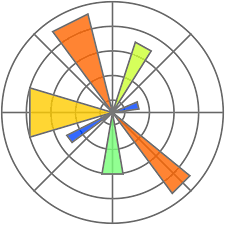
\includegraphics[width=\textwidth,height=1em]{icons/matplotlib-icon.png}
  Matplotlib

  {Matplotlib est une bibliothèque complète pour créer des
  visualisations statiques, animées et interactives en Python.}
\end{itemize}

Formule Statistique

\textbf{Moyenne Mobile Arithmetique}

{On appelle moyenne mobile centrée d'ordre k de la série
\(\{Y_t, t=1,\ldots,n\}\) les Moyennes Mobiles arithmétiques calculées
sur \(k\) valeurs successives.}

\begin{itemize}
\item
  Si k est impaire avec k=2m+1 :\\
  {\(M_{t}(k)\) = \(\frac{1}{k}\sum_{i=m}^{m}Y_{t+i}\)}
\item
  Si k est paire avec k=2m :\\
  {\(M_t(k)\) =
  \(\frac{1}{k}\left[\frac{Y_{t-m}}{2}+ \sum_{i=-m+1}^{m-1}Y_{t+i} + \frac{Y_{t+m}}{2}\right]\)
  }\\
\end{itemize}

\textbf{Moyenne Mobile Exponentielle}

\begin{itemize}
\item
  Formule de la Moyenne Mobile Exponentielle:\\
  \[\large{\bar{x}_t = \alpha\left( x_t + \left(1 - \alpha \right)x_{t-1} + {\left(1 - \alpha \right)}^2x_{t-2} + {\left(1 - \alpha \right)}^3x_{t-3} + \ldots \right)}\]
  \[\large{\bar{x}_t = \sum_{n=0}^{\infty}\alpha{\left(1 - \alpha\right)}^nx_{t-n} }\]
\end{itemize}

\textbf{Oscillateur Stochastiue}

\begin{itemize}
\item
  Formule de la ligne \%K sur une période p:
\item
  \(\%K\) = \({\frac{(C - L)}{(H - L)}}*100\)
\item
  C : c'est le prix de clôture de l'actif.
\item
  L : c'est le prix le plus bas de l'actif sur les N dernères périodes.
\item
  H : c'est le prix le plus élevé de l'actif sur les N dernière
  périodes\\

  \[\begin{cases}
  		\large{L = Y_{min_t}  = min\left( Y_{t-p},Y_{t-p+1},\ldots,Y_{t+p} \right)}\\
  		\\
  		\large{H = Y_{max_t} = max\left( Y_{t-p},Y_{t-p+1},\ldots,Y_{t} \right)}
  		%\item[$ $] $L = Y_{min_t} = min\left( Y_{t-p},Y_{t-p+1},\ldots,Y_{t+p} \right)$\\
  		%\item[$ $] $H = Y_{max_t} = max\left( Y_{t-p},Y_{t-p+1},\ldots,Y_{t+p} \right)$
  	\end{cases}\]
\item
  Formule de la ligne \(\%D\)
\item
  Si k est impaire :

  \(\%D_t(k)\) = \(\frac{1}{k}\sum_{i=m}^{m}\%K_{t+i}\)

  \hfill\break
\item
  Si k est paire :

  \(\%D_t(k)\) =
  \(\frac{1}{k}\left[\frac{\%K_{t-m}}{2}+ \sum_{i=-m+1}^{m-1}\%K_{t+i} + \frac{\%K_{t+m}}{2}\right]\)

  \hfill\break
\end{itemize}

\textbf{Moyenne Mobile Convergence Divergence}

\begin{itemize}
\item
  Formule de la MACD\\
  Soit C et L les périodes respectives des Moyennes Mobiles rapide et
  des Moyennes Mobiles lente.

  \[macd = \bar{x}_C(t)-\bar{x}_L(t)\] \[\begin{cases}
  				\bar{x}_t(C) = 
  					\sum_{n=0}^{C}\alpha{\left(1 - \alpha\right)}^nx_{t-n}\\

  				\bar{x}_t(L) = 
  					\sum_{n=0}^{L}\alpha{\left(1 - \alpha\right)}^nx_{t-n}
  			\end{cases}\]
\item
  Formule de la ligne SIGNALE Soit S la période de la moyenne mobile de
  la ligne SIGNALE \[\begin{cases}
  	\text{Si S est impaire}:\begin{large} \%D_t(k) = \frac{1}{S}\sum_{i=m}^{m}macd_{t+i}\end{large}\\ 
  	\text{Si S est paire} : \begin{large} \%D_t(k) = \frac{1}{S} \left[\frac{macd_{t-m}}{2}+ \sum_{i=-m+1}^{m-1}\%K_{t+i}+ \frac{\%K_{t+m}}{2} \right] \end{large}
  	\end{cases}\]
\end{itemize}

\subsubsection{Profil d'investisseur et paramètres des stratégies de
traing.}\label{profil-dinvestisseur-et-paramuxe8tres-des-stratuxe9gies-de-traing.}

{ Pour déterminer qu'une stratégie est meilleur pour un indice précis
nous devons d'abord déterminer les bons paramètres qui maximise le
rendement de la stratégie. La détermination des meilleurs paramètres
pour chaque stratégies passe par une étape de validation durant laquelle
les meilleur paramètres devrons respecter un certain nombre de critère
de validation élaborer dans le cadre de cette étude. Notons également
que les critère de validation présenter ci-dessous s'adapte à un profil
d'investisseur précis dans le cadre de cette étude.}

\paragraph{Profil d'investissement.}\label{profil-dinvestissement.}

{ Le profil d'investisseur est généralement défini en fonction du niveau
de tolérance au risque financier qu'un investisseur est prêt à assumer,
en comprenant le risque financier comme capacité d'assumer une perte. Il
est déterminée en évaluant des éléments du caractère de l'investisseur
comme la rentabilité qu'il espère obtenir, son objectif
d'investissement, sa tolérance au risque{[}2{]}.}

\begin{itemize}
\item
  \textbf{Objectifs d'investissement.}

  { Les objectifs d'investissement en trading peuvent varier en fonction
  des stratégies et des préférences de chaque individu ou institution.
  Voici quelques types d'objectifs d'investissement courants en trading
  :}

  \begin{enumerate}
  \item
    Objectif de croissance du capital ; L'objectif principal est de
    réaliser des profits en augmentant la valeur du capital investi. Les
    traders cherchent à exploiter les mouvements du marché pour générer
    des rendements positifs.
  \item
    Protéger son patrimoine contre un risque donné grâce à une stratégie
    de couverture ; c'est-à-dire prendre des mesures pour réduire ou
    neutraliser l'impact des fluctuations défavorables sur la valeur
    d'un actif ou d'un portefeuille d'investissement. Cette approche est
    souvent utilisée pour minimiser les pertes potentielles causées par
    des mouvements de marché indésirables{[}7{]}.
  \item
    Spéculer sur les marchés ; c'est-à-dire à faire des paris sur
    l'évolution des prix à la hausse comme à la baisse{[}7{]}.
  \item
    Objectif de revenu régulier : Certains traders cherchent à obtenir
    un revenu régulier en utilisant des stratégies de trading qui visent
    à générer des gains constants à partir de leurs investissements.
  \end{enumerate}
\item
  \textbf{Horizon temporel.}

  Un horizon temporel (ou un horizon d'investissement) correspond à la
  durée totale pendant laquelle un titre est supposé être détenu par un
  investisseur. Les types d'horizons temporels varient de court terme à
  long terme. Certains traders fixent un horizon d'investissement plus
  long car ils disposent de plus de temps pour maintenir leur
  portefeuille investi et ainsi réaliser des bénéfices ou compenser les
  pertes subies. Normalement, avec un horizon à long terme, les
  investisseurs se sentent plus à l'aise pour prendre des décisions
  d'investissement plus risquées et capitaliser sur la volatilité du
  marché. Alors qu'à court terme, comme dans le cas d'un trader
  (négociateur sur séance), les investisseurs doivent veiller à éviter
  les investissements plus risqués (en particulier ceux qui sont proches
  de l'échéance) afin de ne pas subir de pertes significatives{[}8{]}.
  Il s'agit ici d'un facteurs crucial qui influence le choix de notre
  stratégie d'investissement.
\item
  \textbf{Tolérance au risque.}

  { En investissements la tolérance au risque est la capacité et la
  volonté d'un investisseur à assurumer une perte de la valeur de notre
  placement. }

  \begin{enumerate}
  \item
    Prudent : La tolérance au risque et la capacité à l'assumer sont
    toutes deux faibles. Les placements comporteront probablement moins
    d'actions et plus d'obligations ou d'actifs du marché monétaire (qui
    procurent généralement des rendements stables et moins de
    fluctuations de cours)
  \item
    Modéré : La niveaux modéré traduit une tolérance au risque plutôt
    élevée, mais une capacité moindre. Ici les placements pourraient
    comprendre une combinaison d'actions et d'obligations pour une
    approche plus équilibrée.
  \item
    Énergique : Ici votre tolérance au risque est élevée, tout comme
    votre capacité à prendre des risques. Vous acceptez que la valeur de
    vos placements puisse subir de grandes fluctuations au fil du temps.
    Vous rechercherez probablement un potentiel de rendement plus élevé.
    Vos placements sont probablement composés principalement d'actions
    (plutôt que d'obligations) de sociétés de grande et de petite
    taille.
  \end{enumerate}
\end{itemize}

\paragraph{Critères de choix des
paramètres.}\label{crituxe8res-de-choix-des-paramuxe8tres.}

La Stratégie des Moyennes Mobiles se base sur une étude des tendances
des Moyennes Mobiles de courte périodes et de longue périodes. A cet
effet, il existe des périodes standards dans l'utilisation de cette
Stratégie. Ces périodes dépendent de divers facteurs, notamment de la
volatilité des actifs et de l'horizon temporel (court terme : MA5, MA10,
moyen terme : MA50, MA100, long terme : MA200, MA250). Cependant, il est
souvent nécessaire d'adapter ces périodes en fonction des conditions
changeantes du marché et des besoins de l'investisseur. De plus la
stratégie de l'Oscillateur Stochastique et de la moyenne mobile
convergence divergence fait également appelle au calcul de certaine
moyenne mobile. Ainsi, dans l'application de la Stratégie de trading
basée sur les Moyennes Mobiles, et celle de la méthode combiné de
l'Oscillateur stochastique et de la moyenne mobile convergence
divergence nous avons testé différentes combinaisons qui ont permis de
trouver les périodes des Moyennes Mobiles rapide et des Moyennes Mobiles
lentes optimales, permettant d'appliquer efficacement la stratégie de
trading. Il s'avère donc nécessaire de faire un choix logique, cohérent
et robuste suivant toutes les périodes trouvées, nos objectifs
d'investissements, notre horizon temporel et la tolérance au risque.

\begin{itemize}
\item
  \textbf{Simulation}

  La simulation consistera à tester plusieurs combinaisons de périodes
  pour les Moyennes Mobiles arithmétiques dans le cas de la stratégie
  basée sur les Moyennes Mobiles. Nous allons recueillir des
  informations sur le pourcentage de bénéfice réalisé à la suite du
  backtesting, le nombre total de signaux d'achat et de vente obtenus en
  utilisant les combinaisons de périodes, le nombre de transactions
  positives effectuées et le nombre de transactions négatives. Dans le
  cas de la Stratégie combinée de l'Oscillateur Stochastique et de la
  moyenne mobile Convergence Divergence, nous allons recueillir des
  informations sur le bénéfice, le nombre de transactions positives
  effectuées et le nombre de transactions négatives, ainsi que les
  combinaisons de périodes utilisées pour calculer les moyennes
  exponentielles, la ligne de signal et la ligne de l'Oscillateur
  Stochastique.

  Notre étude encourage l'investissement à cout et à long terme, ainsi
  donc nos simulations se feront pour des valeurs de la période courte
  de 20 à 50 et pour des valeurs de la période longue de 50 à 150. À la
  fin de la simulation, nous choisirons les périodes ayant généré un
  bénéfice d'au moins 20\%, un taux de transactions positives élevé et
  robuste.
\item
  \textbf{Taux de réussite des transactions.}

  Une transaction est réussite lorsque le prix d'achat de l'actif est
  inférieur au prix de ventes. En d'autre termes, la transaction est
  réussite lorsque nous réalisons un bénéfice. Il arrive en effet lors
  de la génération des signaux que l'on obtiennent des faux signaux
  causé par un retard ,une grand fluctuation du marché etc... Le taux de
  réussites des transaction mesure donc la performance de la combinaison
  de période utilisée en ce basant sur le nombre de transaction réussi
  par rapport au nombre total de transactions effectuer.
\item
  \textbf{Robustesse}

  {La Robustesse est la capacité à ne pas être perturbé par une
  modification dans une petite partie des données. Une période est
  résistante lorsque la rentabilité produite par la période n'est pas
  très éloigner des rentabilités produites par les périodes
  avoisinantes.}
\end{itemize}

\paragraph{Outils d'analse des
données}\label{outils-danalse-des-donnuxe9es}

\begin{itemize}
\item
  \textbf{Les tendances}

  La tendance est considérée comme étant la pierre angulaire de
  l'analyse technique par les traders, et dénote la direction d'un
  marché à un moment donné indiquant la tendance de la variation des
  prix. On distingue trois catégories de tendances à savoir, la tendance
  haussière, la tendance baissière et la tendance neutre.

  Une tendance haussière en bourse est une direction générale à la
  hausse des prix d'un actif sur une période donné. Elle se produit
  lorsque les prix d'un actif augmente régulièrement sur une période de
  temps donnée. Certains investisseur optimistes achètent souvent dans
  une tendance haussière dans l'espoir de réaliser des gains à mesure
  que le prix continue d'augmenter. Une tendance à la baisse est une
  situation boursière dans laquelle le prix d'un actif financier baisse
  pendant une certaine période{[}5{]}. Une tendance latéral se produit
  lorsque le prix d'un actif évolue horizontalement, sans tendance nette
  à la hausse ou à la baisse. Une tendance en dent de scie se
  caractérise se caractérise par des creux et des sommets qui se forment
  à des niveaux différents sans direction claire. Une tendance est un
  inversion de l'évolution des cours d'un actif : lorsqu'une tendance
  haussière se transforme en tendance baissière et vise versa.
\item
  \textbf{Les niveaux de support et de résistance.}

  Les niveaux de résistance et de support illustre la manière dont les
  forces de l'offre et de la demande interagissent pour déterminer le
  prix en vigueur d'un actifs sous-jacent{[}4{]}. La résistance est une
  ligne qui relie les sommets des points les plus hauts de la courbe des
  actifs. Le support est une ligne qui relie les sommets des points les
  plus bas de la courbe. Si une ligne touche au moins trois points, elle
  devient significative. Plus les cours viendront toucher les lignes de
  résistance et de support, plus elles résisteront aux hausses et aux
  chutes du cours des actions. Les Lignes de résistances et de support
  peuvent être utilisées pour délimiter les zones potentielles où les
  prix peuvent rencontrer des changements de directions.

  Lorsque les cours arrivent finalement à traverser la résistance cela
  voudrait dire qu'ils ont accumulé assez de force pour traverser la
  résistance et qu'un changement significatif existe. Si les cours
  traversent le support cela implique une diminution potentiellement
  significative du cours de l'actifs.
\item
  \textbf{Les Moyennes Mobiles.}

  {La moyenne mobile est une ligne de tendance qui donne une idée de
  l'évolution des cours du marché. À chaque point de la moyenne mobile,
  la valeur est un indicateur du prix moyen sur une période donnée.
  Parfois il s'agit de la moyenne mobile arithmétique, d'autres fois ce
  sont des Moyennes Mobiles plus complexes qui sont utilisées, comme la
  moyenne mobile exponentielle. La configuration et la mise en œuvre de
  cet indicateur nécessitent un paramètre très important, qui est la
  période de temps. En trading, les Moyennes Mobiles sont utilisées pour
  générer des signaux d'achat et des signaux de vente. Dans la plupart
  des cas, deux Moyennes Mobiles sont utilisées dans le but de générer
  les signaux : la moyenne mobile rapide et la moyenne lente.}

  {La moyenne mobile rapide, comparativement à la moyenne mobile lente,
  est calculée sur une période plus courte. Vient donc une question
  primordiale qui est comment choisir la période des deux Moyennes
  Mobiles qui répond au mieux à nos données? Pour la moyenne mobile
  rapide, on peut choisir une moyenne mobile qui sert de support à la
  correction d'une remontée franche arrivant après un plus bas, et pour
  la moyenne mobile lente, le double de la période de la moyenne mobile
  rapide. {[}1{]} Étant donné que chaque valeur sur le marché peut avoir
  ses propres caractéristiques uniques, indépendamment des tendances
  générales du marché, il est nécessaire d'utiliser plusieurs périodes
  de Moyennes Mobiles pour trouver la période qui convient le mieux à
  l'analyse du titre spécifié. Par ailleurs, il faut garder à l'esprit
  de toujours garder une différence considérable entre les périodes des
  Moyennes Mobiles rapides et les périodes des moyennes lentes, pour
  éviter que les courbes ne se chevauchent et donc donnent des signaux
  contradictoires. En effet, suivant les valeurs de la différence entre
  la période lente et la période rapide, plus la différence est grande,
  plus les Moyennes Mobiles s'éloigneront les unes des autres. Cette
  différence est l'un des paramètres permettant de définir le profil
  d'investissement (spéculation, investissement à moyen terme,
  investissement à long terme). }
\item
  \textbf{Stratégie des moyennes mobile.}

  {La stratégie des Moyennes Mobiles utilise les Moyennes Mobiles
  arithmétiques sur deux différentes périodes : la moyenne mobile lente
  (moyenne longue) et la moyenne mobile rapide (courte). En effet, la
  moyenne mobile arithmétique est un indicateur technique utilisé pour
  lisser les données de prix sur une période donnée. Son objectif
  principal est de fournir une estimation de la tendance générale des
  prix en filtrant les fluctuations. Suivant les différents croisements
  des deux Moyennes Mobiles, on peut détecter des signaux d'achat et de
  vente. Ainsi, lorsque la moyenne mobile rapide croise et dépasse la
  moyenne mobile lente, alors le marché est en tendance haussière ce qui
  est un signal d'achat. Par contre, quand la moyenne mobile rapide
  croise et est inférieure à la moyenne mobile lente, alors le marché
  est en tendance baissière et cela implique un signal de vente. Si les
  deux moyennes sont confondues, nous sommes en range. La création de
  cette stratégie est généralement attribuée à \textbf{Charles H. Dow},
  un journaliste financier américain et fondateur du Dow Jones \&
  Company. Il est l'un des pionniers de l'analyse technique des marchés
  financiers et de l'utilisation des Moyennes Mobiles.}
\item
  \textbf{Strategie de la Moyenne mobile convergence divergence.}

  {L'indicateur MACD (Moving Average Convergence Divergence) est un
  indicateur de suivi de tendance utilisé pour localiser les tendances
  du marché. Il est composé d'un histogramme de deux lignes calculées à
  partir des Moyennes Mobiles exponentielles et d'une ligne MACD et
  d'une ligne signal. Les deux lignes de Moyennes Mobiles Exponentielles
  sont calculées sur les cours de clôture. En effet, la Moyenne Mobile
  Exponentielle est un indicateur technique qui permet de lisser les
  cours des actifs en affectant plus de poids aux prix les plus récents
  tout en diminuant progressivement le poids des prix plus anciens. La
  ligne MACD est le résultat de la différence entre les Moyennes Mobiles
  rapides qui sont de courtes périodes et la moyenne mobile lente qui
  est de longue période. Une MACD positive indique une tendance
  haussière et une MACD négative indique une tendance baissière. La
  ligne signal est la moyenne mobile arithmétique de la ligne MACD.
  Cette ligne lisse la MACD et permet de générer les signaux d'achat et
  de vente. Ainsi, suivant les valeurs de la ligne signal et de la ligne
  MACD, lorsque la ligne MACD croise la ligne de signal et la dépasse,
  cela génère un signal d'achat et dans le cas où la ligne MACD croise
  la ligne signal et passe en-dessous de celle-ci, cela génère un signal
  de vente. La MACD a été développée par \textbf{Gérald Appel}, un
  analyste financier et trader américain connu pour ses contributions à
  l'analyse technique. Il faut noter que l'indicateur est le résultat de
  nombreuses contributions et améliorations apportées par divers
  professionnels de l'analyse technique au fil des ans. Cependant, étant
  donné que la Moyenne Mobile est un type d'indicateur technique qui se
  base sur des données historiques pour générer des signaux (indicateur
  retard), il est donc par conséquent lent à réagir aux changements de
  prix comparativement aux indicateurs avancés qui anticipent les
  mouvements futurs des prix. Pour cela, il est important de combiner la
  MACD avec d'autres indicateurs afin de confirmer les signaux.}
\item
  \textbf{Strategie de l' oscillateur stochastique.}

  {L'oscillateur stochastique est un indicateur qui évalue les
  conditions de surachat et de survente du marché. Le stochastique est
  basé sur le fait que lorsque les prix suivent une tendance haussière,
  les prix de fermeture tendent à se rapprocher du niveau supérieur de
  l'écart des prix. de même lorsque la tendance des prix est en baisse,
  les prix de fermeture tendent à se rapprocher du niveau inférieur de
  l'écart des prix. Pour cela, il fait appel à deux lingnes nommées \%K
  et \%D. Le \%D est le plus plus important dans le sens ou c'est lui
  qui donne le signal. Ces lignes permettent de savoir si le marché est
  dans un état de surachat ou dans un état de survente{[}3{]}. En effet,
  la ligne \%K est la ligne principale de l'oscillateur stochastique.
  Elle représente la position actuelle du prix de clôture par rapport à
  un échantillon de prix sur une période donnée. La ligne \%D, quant à
  elle, est la moyenne mobile arithmétique de la ligne \%K sur une autre
  période. Cette ligne est lissée afin de donner une meilleure
  indication sur les conditions du marché. Suivant les deux lignes, une
  valeur de \%K et de \%D de moins de 30\% indique que nous sommes dans
  un état de survente, et une valeur de plus de 70\% indique un marché
  dans un état de surachat. Développé par \textbf{George C. Lane} vers
  les années 1950, l'oscillateur stochastique est utilisé pour
  identifier les changements potentiels dans les tendances et pour
  confirmer les signaux générés par d'autres indicateurs.}
\end{itemize}

\paragraph{\texorpdfstring{Critère de decision
}{Critère de decision }}\label{crituxe8re-de-decision}

\begin{itemize}
\item
  \textbf{Le Backtesting.}

  {Le Backtesting est une façon d'analyser la performance potentielle
  d'une stratégie de trading en l'appliquant à des données historiques
  réelles. C'est un outil qui aide à choisir la stratégie présentant le
  meilleur résultat. Cette stratégie se base sur l'idée selon laquelle
  une stratégie ayant donné de meilleurs résultats sur des données
  passées est susceptible de le faire également dans les conditions
  actuelles ou futures du marché. En effet, le Backtesting permet de
  tester les stratégies tout en ajustant les paramètres afin d'obtenir
  les meilleurs résultats. Les tests sont réalisés très rapidement et
  sans risquer le capital.}
\end{itemize}

\paragraph{\texorpdfstring{Limite de l'étude.
}{Limite de l'étude. }}\label{limite-de-luxe9tude.}

{Notre étude compare uniquement les performances de deux stratégies de
trading sur les indices BRVM-Agriculture et BRVM-Service Publique.
Malheureusement, les résultats de notre étude ne peuvent pas être
utilisés pour d'autres indices ou pour d'autres titres sur d'autres
marchés, y compris même celui de la BRVM. De plus, les périodes
utilisées pour les calculs de moyenne mobile sont de plus de 20 jours,
ce qui n'est pas convenable pour les traders spéculateurs. Il faut noter
que le Backtesting, bien qu'il permette de trouver la stratégie la plus
performante, ne garantit cependant pas la fiabilité de celle-ci sur les
données futures du marché.}

\section{ANALYSE DES RESULTATS, VERIFICATION ET
SOLUTIONS}\label{analyse-des-resultats-verification-et-solutions}

\subsection{Collecte des données et analyse des
résultats}\label{collecte-des-donnuxe9es-et-analyse-des-ruxe9sultats}

\subsubsection{Présentation des données et analyse des
résultats}\label{pruxe9sentation-des-donnuxe9es-et-analyse-des-ruxe9sultats}

\paragraph{Analyse descriptive.}\label{analyse-descriptive.}

{Encore appelé statistique descriptive, l'analyse descriptive permet de
décrire et de résumer les caractéristique essentielles d'un ensemble de
données. En analyse technique, en plus des statistiques élémentaire on
peut faire également une analyse des tendances pour comprendre les
mouvements de prix d'un actif financier au fil du temps. De plus une
analyse des niveaux de résistances et de support permet de fournir des
repères pour déterminer les zones ou les prix sont susceptible de réagir
ou potentiellement inverser leur direction.}

\begin{itemize}
\item
  \textbf{L'indice BRVM-Services-Publics.}

  {L'analyse descriptive des données de la BRVM-Agriculture, basée sur
  les données antérieures de la Bourse régionale des valeurs
  immobilières sur la période allant du \textbf{16 juin 2020} au
  \textbf{15 mai 2023}, révèle de nombreux points importants. En effet,
  la valeur moyenne de cet indice durant cette période s'élève à 439,55,
  ce qui indique un niveau de prix autour duquel les prix tendent à se
  regrouper. L'écart type de 47,60 suggère que les prix de clôture sont
  légèrement dispersés par rapport à la moyenne, ce qui explique une
  certaine stabilité dans les fluctuations. Le prix minimum atteint
  durant cette période est de 328,64 tandis que le prix maximum atteint
  est de 528,59. En étudiant les quartiles, nous pouvons remarquer que
  25\% des prix sont inférieurs à 397,54, tandis que 75\% des prix de
  clôture sont inférieurs à 475,15, ce qui montre une distribution des
  prix légèrement asymétrique. Avec une valeur de 449,34, la médiane
  indique que la moitié des prix sont inférieurs à cette valeur. Suivant
  les niveaux de résistance et de support sur la figure ci-dessous, nous
  pouvons remarquer qu'aucune ligne de support ni de résistance ne
  respecte la "règle des trois touches", qui suggère que la résistance
  et le support sont valides lorsqu'ils ont été touchés au moins trois
  fois sans être traversés par la courbe des prix.}

  { En général, nous pouvons noter une légère augmentation du cours de
  l'indice durant la période allant de juin 2020 à mai 2023. Cette
  augmentation traduit une appréciation positive de la valeur par les
  investisseurs ou simplement une demande de plus en plus importante
  pour cette valeur.}

  \begin{figure}
  \hypertarget{fig:Tendancesux20deux20lux27indiceux20BRVM-Services-Publics}{%
  \centering
  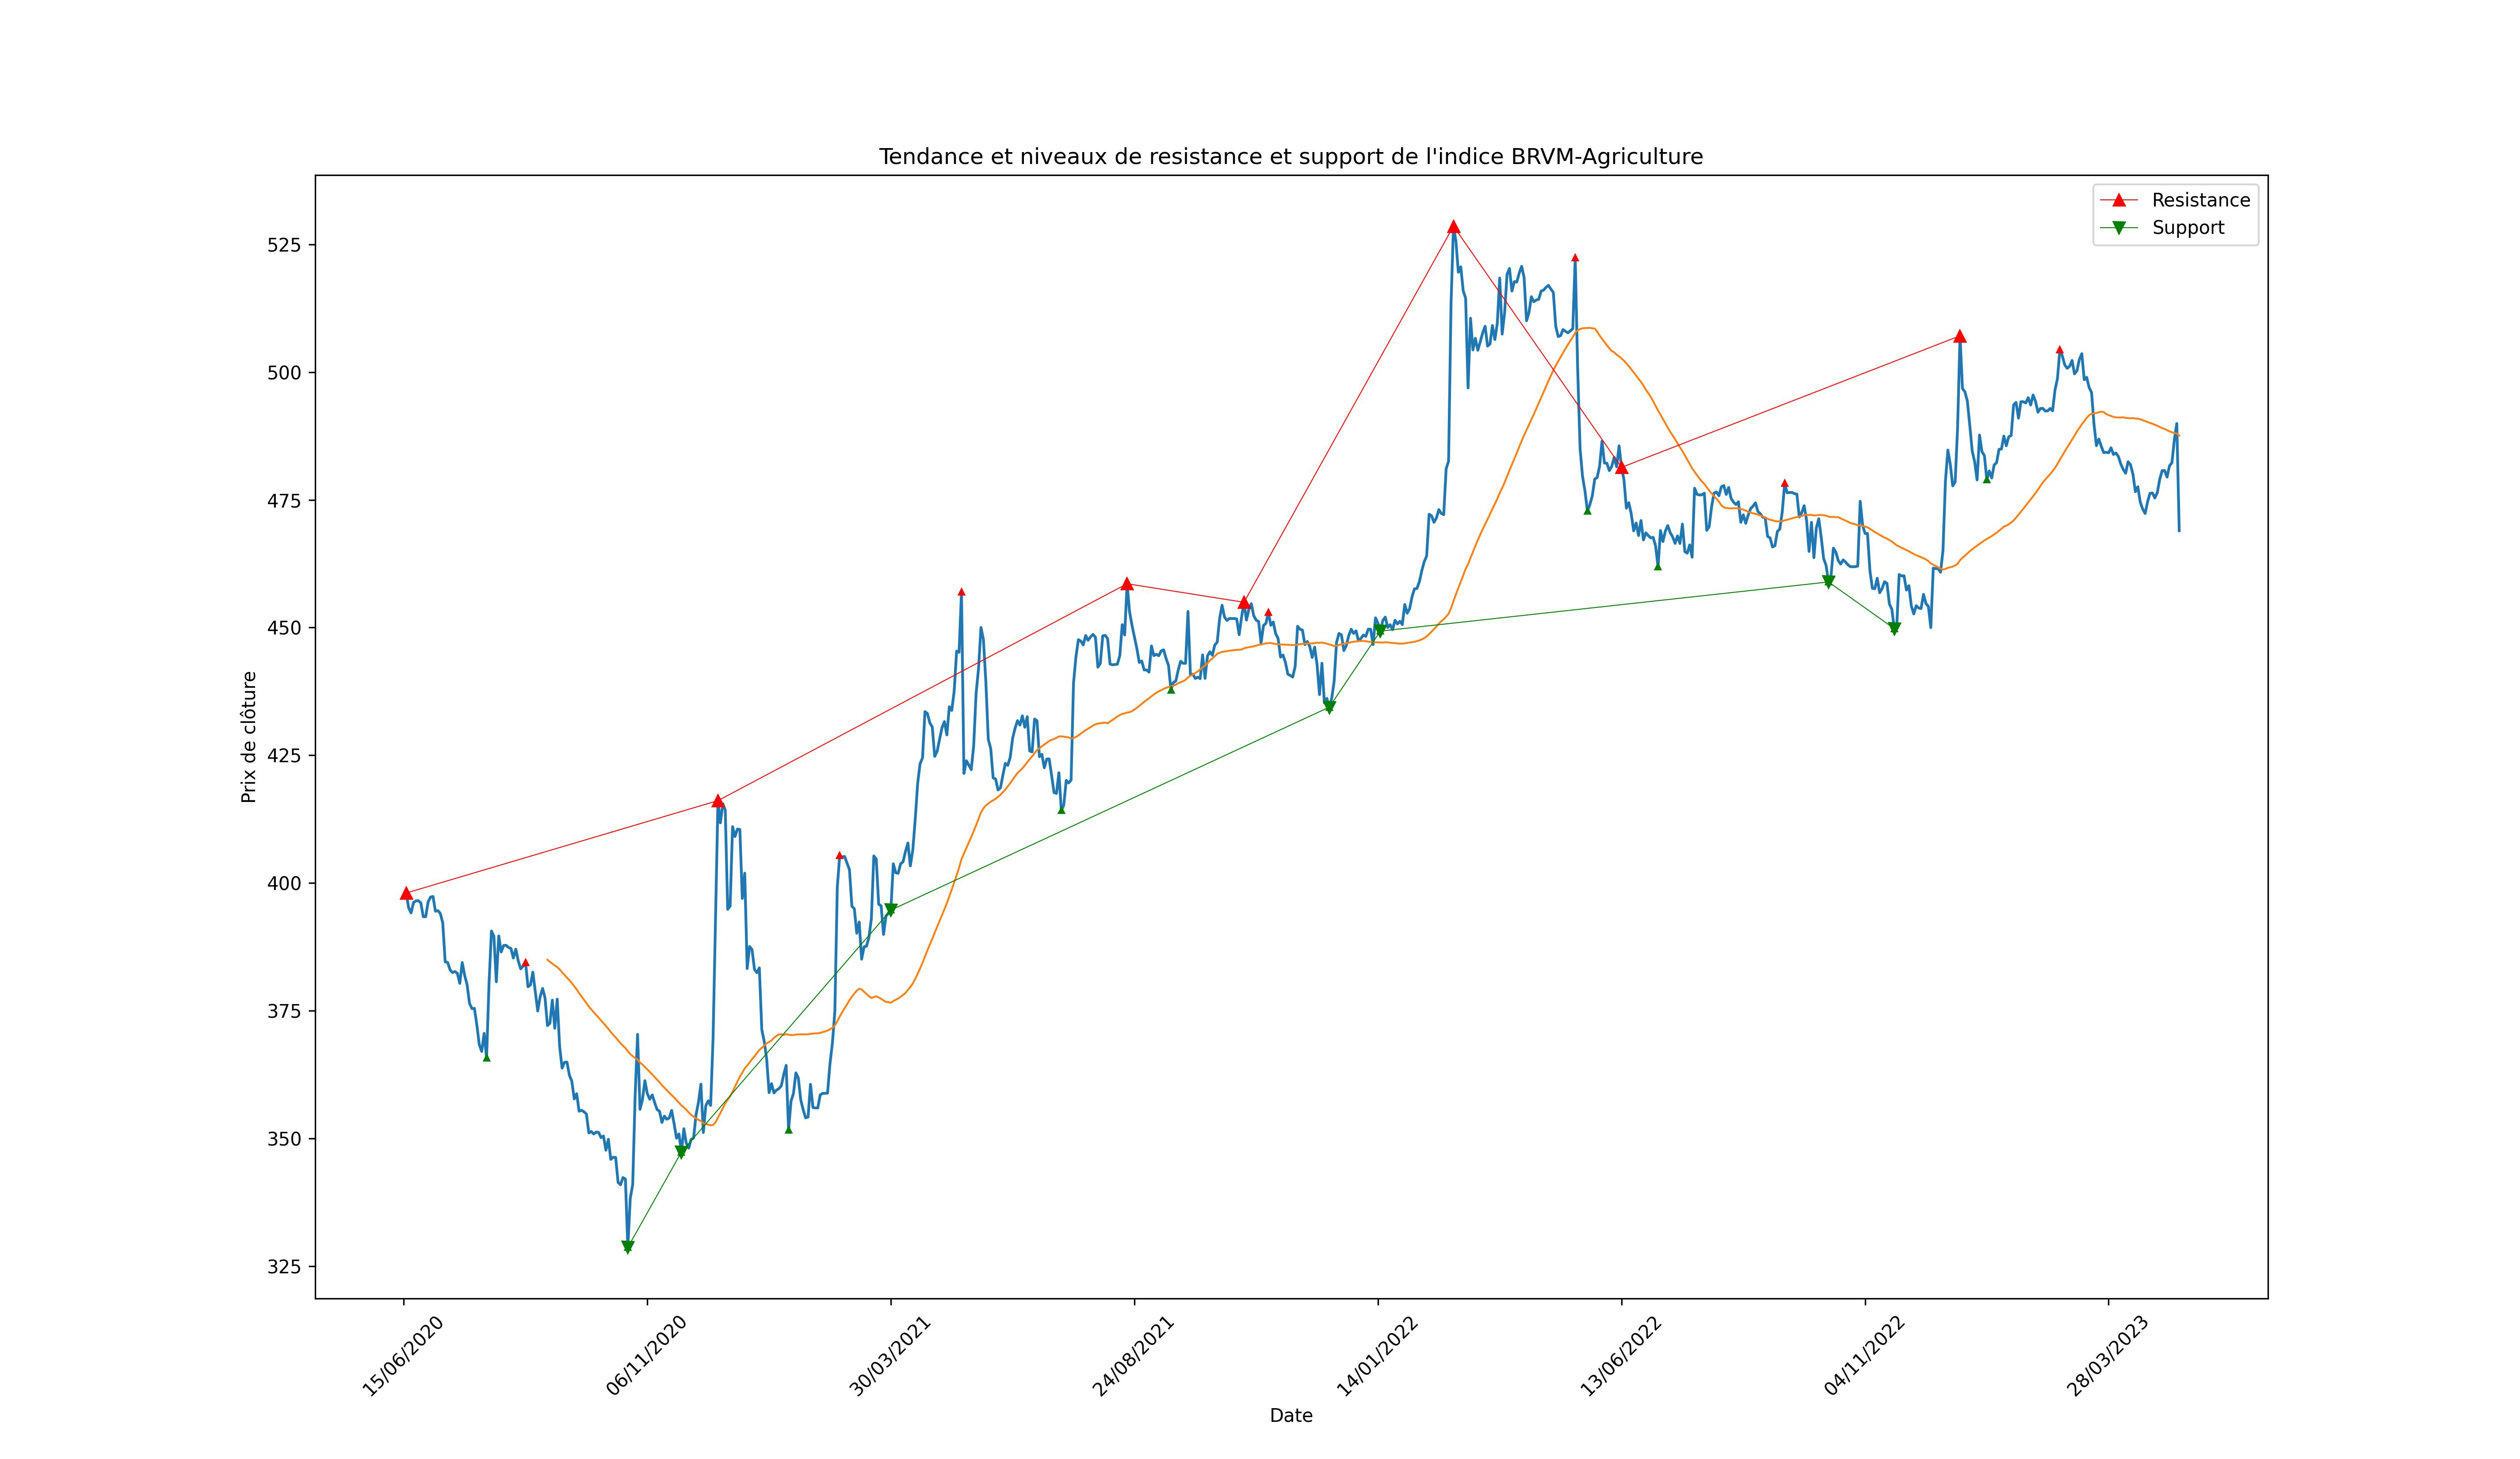
\includegraphics{img/public_tendance.jpg}
  \caption{Tendances de l'indice
  BRVM-Services-Publics}\label{fig:Tendancesux20deux20lux27indiceux20BRVM-Services-Publics}
  }
  \end{figure}
\item
  \textbf{BRVM-Agriculture}

  {L'analyse descriptive de l'indice BRVM-Agriculture sur la période du
  \textbf{16 juin 2020} au \textbf{15 mai 2023} révèle principalement
  une très grande augmentation du cours de la valeur. En effet, à la
  date du 15 mai 2023, le prix de l'indice BRVM-Agriculture valait 65,92
  pour atteindre 248,05 Fcfa le 15 mai 2023. Autrement dit, la valeur
  vaut plus de 3,5 fois sa valeur initiale. Par ailleurs, le prix
  minimum atteint durant cette période est de 55,40 Fcfa enregistré le
  \textbf{mercredi 05 août 2020} et un maximum de 349,65 Fcfa atteint le
  \textbf{lundi 16 mai 2022}. En moyenne, le prix de clôture de la
  "BRVM-Agri" durant cette période tourne autour de 206,82 Fcfa. L'étude
  des quartiles révèle que 25\% des cours sont inférieurs à 109,59 Fcfa
  et 75\% sont inférieurs à 287,00 Fcfa. En plus d'un écart type de
  95,12, qui suggère une légère distribution par rapport à la moyenne,
  nous pouvons remarquer graphiquement une évolution des cours très
  progressive et sans changement brusque. Suivant les niveaux de
  résistance et de support, nous pouvons remarquer que seulement la
  troisième résistance ne respecte pas la "règle des trois points
  touchés". En effet, nous pouvons observer que la résistance qui
  commence vers le 09 novembre 2020 est touchée cinq fois par la courbe
  de l'évolution des cours de la valeur avant d'être traversée plutôt au
  sixième pic vers le 25 août 2022 pour atteindre un nouveau record de
  259,08 Fcfa le \textbf{mardi 26 octobre 2021}, ce qui valide la
  résistance précédente.}

  \begin{figure}
  \hypertarget{fig:Tendanceux20deux20lux27indiceux20BRVM-Agriculture}{%
  \centering
  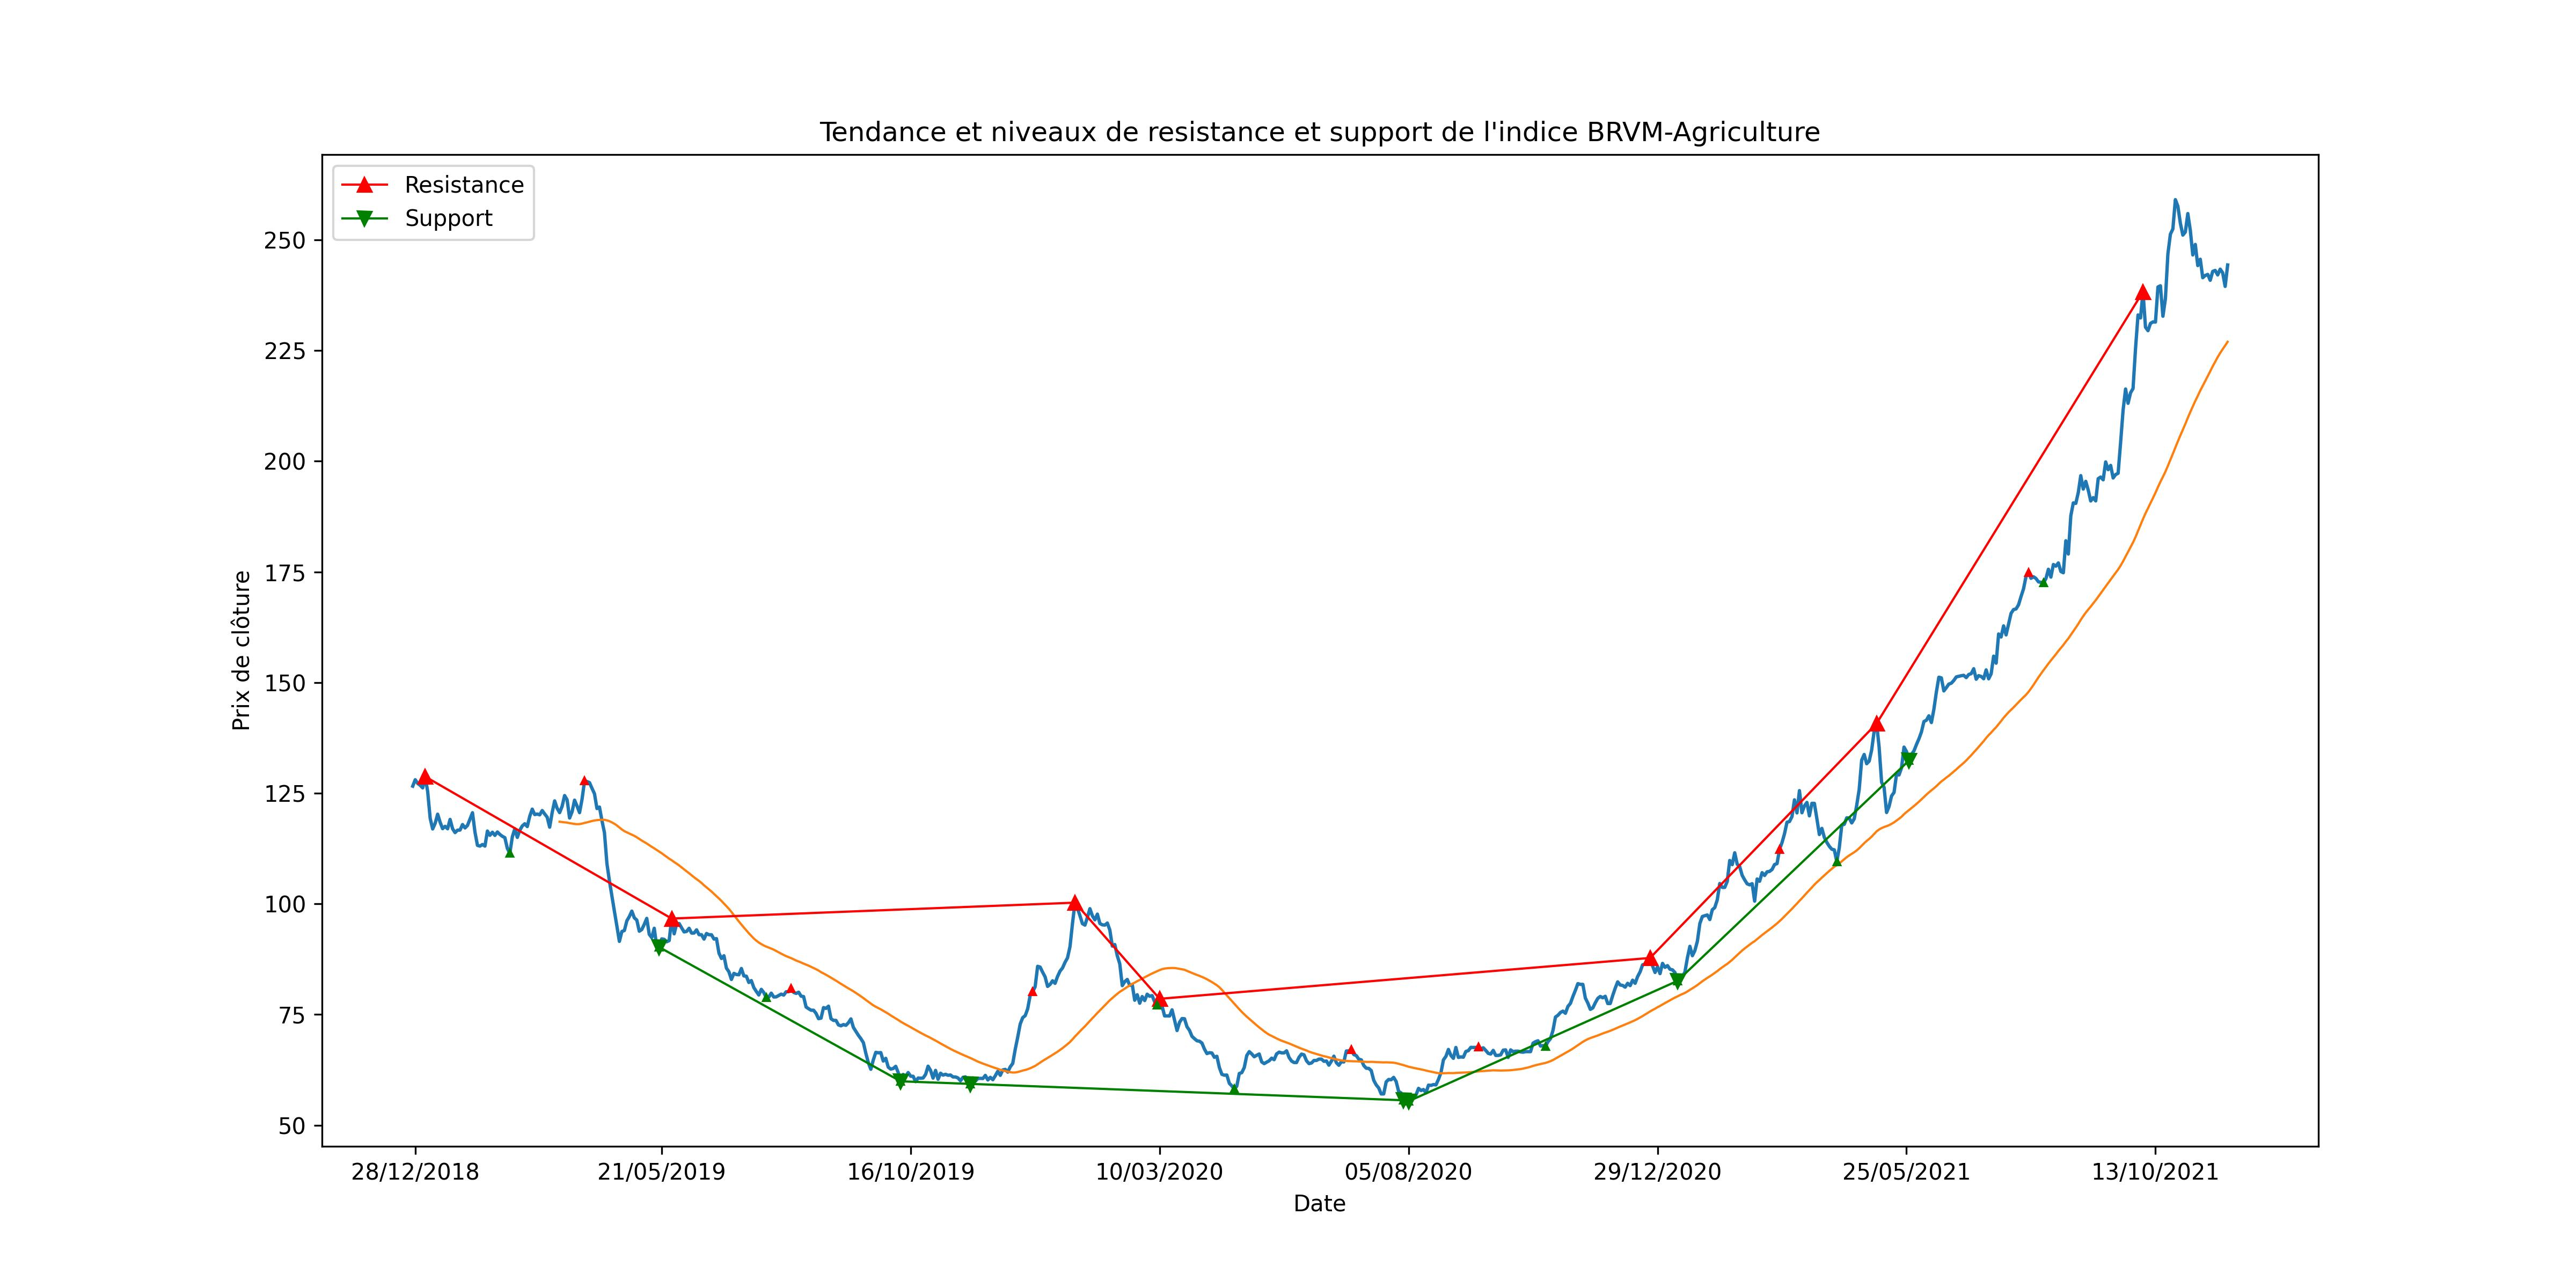
\includegraphics{img/agri_tendance.jpg}
  \caption{Tendances de l'indice
  BRVM-Agriculture}\label{fig:Tendanceux20deux20lux27indiceux20BRVM-Agriculture}
  }
  \end{figure}
\end{itemize}

\paragraph{Analyse des resultats.}\label{analyse-des-resultats.}

\textbf{Profil d'investissement.}

\begin{itemize}
\item
  \textbf{Objectifs d'investissement :} Dans cette étude ou nous
  cherchons la meilleur stratégie de trading pour chaque indices
  (BRVM-agriculture et BRVM-Service-Publics), notre objectif est de
  pouvoir acheter ces valeurs à un moins cours et les revendre plus
  chère. Notre objectif d'investissement est donc la \textbf{croissance
  du capital}.
\item
  \textbf{Horizon temporel :} Pour l'application des stratégies de
  trading nous prévoyons de conserver la valeur pendant une période
  assez longue. Dans cette étude nous faisons le choix d'un
  investissement à moyen terme.
\item
  \textbf{Tolérance au risque :} Dans cette étude, nous effectuons des
  opérations de trading sur les marchés d'indices boursiers. À chaque
  signal d'achat, nous achetons la valeur si nous ne possédons pas du
  stock puis nous revendons toute la valeur au prochain signal de vente.
  Nous acceptons donc que la valeur de nos placement puisse subir de
  grandes fluctuations au fil du temps. De plus nous recherchons une
  stratégie avec d'un potentiel de rendement élever. Nous avons donc un
  profil d'inverstisseur 'Energique'.
\end{itemize}

\textbf{Paramètres des Stratégies de trading.}

Afin de déterminer la combinaison de périodes qui maximise le bénéfice
pour la Stratégie des Moyennes Mobiles, des simulations ont été
effectuées sur un ensemble de couples de périodes afin de recueillir les
informations sur chaque période. Des informations telles que le nombre
de signaux positifs, le nombre de signaux négatifs, le nombre de
transactions positives, le nombre de transactions négatives, et le taux
de bénéfice réalisé sur cette combinaison de périodes. A cet effet, les
Moyennes Mobiles ont été testées sur un intervalle de \textbf{10 à 54}
pour la période "rapide" et de \textbf{24 à 100} pour la période
"lente".

Au total, nous avons enregistré \textbf{3465} observations. Parmi ce
grand nombre de possibilités, se trouve une et une seule combinaison de
périodes qui répond le mieux à nos données et en même temps à nos
critères de choix. Cependant, il est important de noter que suite aux
simulations le maximum de bénéfice pour l'indice BRVM-Agriculture a été
obtenu grâce aux périodes 35 pour la moyenne mobile lente et 34 pour la
moyenne mobile rapide, avec \textbf{446,531\%} de bénéfice pour 16
transactions réussies sur 21 transactions au total. En ce qui concerne
l'indice BRVM-Services-Publics, le plus grand taux de bénéfice est
observé avec la période 30 pour la moyenne mobile lente et 32 pour la
moyenne mobile rapide, avec un total de \textbf{44,009\%} de bénéfice
pour 14 transactions réussies sur 25. Dans la suite, nous présenterons
l'application des différents critères de sélection de périodes ainsi que
les filtrages.

\begin{itemize}
\item
  \textbf{Paramètres pour la stratégie des Moyennes Mobiles.}

  \begin{itemize}
  \item
    Difference entre période.

    {Il est conseillé que la moyenne mobile lente fasse au moins le
    double de la moyenne mobile rapide. Pour cela, nous allons prendre
    en considération uniquement les combinaisons de périodes dont la
    période "lente" fait au moins le double de la période "rapide". À la
    suite de cette sélection, il restait un total de \textbf{1675}
    observations (dans les deux cas). }
  \item
    Taux de réussite des transactions.

    {Une transaction est réussie lorsque le prix de vente de l'actif est
    supérieur à son prix d'achat. Ici, nous allons sélectionner
    uniquement les observations ayant un taux de transactions réussies
    de plus de \textbf{80\%}. Suite à ce filtrage, il ne restait plus
    que \textbf{6} observations pour les périodes de l'indice
    BRVM-Agriculture et \textbf{37} observations pour les périodes de
    l'indice BRVM-Services-Publics.}
  \item
    Taux de bénéfice.

    {Dans ce niveau de filtrage, nous allons prélever la période qui a
    généré le pourcentage de bénéfice le plus élevé parmi les 6
    observations dans le cas de l'indice BRVM-Agriculture et les 37
    observations en ce qui concerne l'indice BRVM-Services-Publics. Dans
    le cas de l'indice BRVM-Agriculture, nous pouvons observer un
    maximum de bénéfice de \textbf{380,184\%} avec les périodes 27 et
    54, et un maximum de bénéfice de \textbf{19,241\%} avec les périodes
    49 et 100 pour l'indice BRVM-Services-Publics.}
  \item
    Robustesse.

    {Ce niveau est le plus important parmi nos filtrages. En effet, nous
    allons vérifier si une légère modification des périodes citées plus
    haut affecte la rentabilité et le nombre de taux de transaction de
    la stratégie.}

    \textbf{"BRVM-agri"}

    \begin{longtable}[]{@{}lllll@{}}
    \caption{Période voisins du couple (27,54) pour la
    BRVM-agri}\tabularnewline
    \toprule\noalign{}
    Longue & Courte & Bénefice & Positive & Négative \\
    \midrule\noalign{}
    \endfirsthead
    \toprule\noalign{}
    Longue & Courte & Bénefice & Positive & Négative \\
    \midrule\noalign{}
    \endhead
    \bottomrule\noalign{}
    \endlastfoot
    53 & 26 & 369.535 & 2 & 1 \\
    54 & 26 & 363.157 & 2 & 1 \\
    55 & 26 & 357.975 & 2 & 1 \\
    53 & 27 & 361.161 & 2 & 1 \\
    54 & 27 & 380.18 & 2 & 0 \\
    55 & 27 & 349.852 & 2 & 1 \\
    53 & 28 & 354.71 & 2 & 1 \\
    54 & 28 & 352.48 & 2 & 1 \\
    55 & 28 & 347.417 & 2 & 1 \\
    \end{longtable}

    {En analysant le tableau ci-dessus, nous pouvons remarquer de très
    petites variations dans le taux de bénéfice, notamment au niveau des
    couples de périodes (28,55), (54,28), (53,28) et (55,27). De plus,
    pour toutes les périodes avoisinant le couple (27,53), nous
    observons un taux de réussite de transaction de 2 sur trois, soit
    \textbf{66,66\%} de transactions réussies. Ainsi, le couple de
    périodes (27,53) n'est pas robuste. Nous allons maintenant chercher
    le couple de périodes ayant donné le plus grand taux de bénéfices
    pour un taux de réussite de transaction d'au moins \textbf{75\%}
    pour au moins trois transactions réussies.}

    \begin{longtable}[]{@{}lllll@{}}
    \caption{Période voisins du couple (24,56) pour la
    BRVM-agri}\tabularnewline
    \toprule\noalign{}
    Longue & Courte & Bénefice & Positive & Négative \\
    \midrule\noalign{}
    \endfirsthead
    \toprule\noalign{}
    Longue & Courte & Bénefice & Positive & Négative \\
    \midrule\noalign{}
    \endhead
    \bottomrule\noalign{}
    \endlastfoot
    55 & 23 & 352.283 & 3 & 1 \\
    56 & 23 & 355.751 & 3 & 1 \\
    57 & 23 & 374.073 & 3 & 1 \\
    55 & 24 & 364.412 & 3 & 1 \\
    56 & 24 & 367.167 & 3 & 1 \\
    57 & 24 & 376.914 & 3 & 1 \\
    55 & 25 & 365.003 & 3 & 1 \\
    56 & 25 & 361.049 & 2 & 1 \\
    57 & 25 & 361.175 & 3 & 1 \\
    \end{longtable}

    {De l'analyse du tableau ci-dessus, nous remarquons qu'une légère
    modification de la période de la moyenne mobile lente et de la
    moyenne mobile courte n'a presque pas d'effet sur le taux de
    bénéfice de la stratégie. En ce qui concerne les taux de
    transaction, nous remarquons qu'il n'y a pas de modification dans le
    nombre total de transactions effectuées et que le nombre de
    transactions négatives reste le même. En effet, cette transaction
    négative est causée par une fluctuation inhabituelle des cours
    observée entre le 26 juillet 2022 et janvier 2023. Mais au vu des
    observations, nous pouvons dire que le couple de périodes (24,56)
    est robuste dans le cadre de l'application de la stratégie de
    trading basée sur les moyennes sur la BRVM-Agri.}

    \textbf{"BRVM-Service-Publics"}

    \begin{longtable}[]{@{}lllll@{}}
    \caption{Période voisins du couple (49,100) pour la
    BRVM-Service-Publics}\tabularnewline
    \toprule\noalign{}
    Longue & Courte & Bénefice & Positive & Négative \\
    \midrule\noalign{}
    \endfirsthead
    \toprule\noalign{}
    Longue & Courte & Bénefice & Positive & Négative \\
    \midrule\noalign{}
    \endhead
    \bottomrule\noalign{}
    \endlastfoot
    99 & 48 & 18.714 & 3 & 0 \\
    100 & 48 & 18.756 & 3 & 0 \\
    101 & 48 & 18.756 & 3 & 0 \\
    99 & 49 & 17.827 & 3 & 0 \\
    100 & 49 & 19.241 & 3 & 0 \\
    101 & 49 & 12.727 & 2 & 1 \\
    99 & 50 & 17.072 & 3 & 0 \\
    100 & 50 & 11.838 & 2 & 1 \\
    101 & 50 & 11.131 & 2 & 1 \\
    \end{longtable}

    {D'après l'analyse du tableau, on remarque un léger changement du
    taux de bénéfice aux alentours du couple de périodes (38 ; 94),
    notamment aux couples (50,101) et (50,100) où le bénéfice descend
    jusqu'à 11\%. Par contre, on peut observer une variation du nombre
    de transactions, notamment des transactions négatives. Nous allons
    maintenant chercher le couple de périodes ayant donné le plus grand
    taux de bénéfices pour un taux de réussite de transaction d'au moins
    \textbf{75\%} pour au moins trois transactions réussies.}

    \begin{longtable}[]{@{}lllll@{}}
    \caption{Période voisins du couple (49,98) pour la
    BRVM-Service-Publics}\tabularnewline
    \toprule\noalign{}
    Longue & Courte & Bénefice & Positive & Négative \\
    \midrule\noalign{}
    \endfirsthead
    \toprule\noalign{}
    Longue & Courte & Bénefice & Positive & Négative \\
    \midrule\noalign{}
    \endhead
    \bottomrule\noalign{}
    \endlastfoot
    97 & 48 & 12.799 & 3 & 0 \\
    98 & 48 & 19.083 & 3 & 0 \\
    99 & 48 & 18.714 & 3 & 0 \\
    97 & 49 & 17.62 & 3 & 0 \\
    98 & 49 & 18.015 & 3 & 0 \\
    99 & 49 & 17.827 & 3 & 0 \\
    97 & 50 & 18.721 & 3 & 0 \\
    98 & 50 & 18.532 & 3 & 0 \\
    99 & 50 & 17.072 & 3 & 0 \\
    \end{longtable}

    {Le couple de périodes (49,98) n'a présenté aucun changement du
    nombre de transactions positives ou négatives pour ses périodes
    voisines. De plus, il n'y a pas une grande variation du taux de
    bénéfice, sauf pour la période 97 pour la moyenne mobile lente et 48
    pour la moyenne mobile rapide, où le bénéfice est descendu à 12\%.
    Au vu de ces observations, nous pouvons déduire que le couple de
    périodes (49,98) est robuste dans le cadre de l'application de la
    stratégie de trading basée sur les moyennes sur la
    BRVM-Services-Publics.}
  \end{itemize}
\item
  \textbf{Paramètres pour la stratégie combiné de l'Oscillateur
  Stochastique et de la moyenne mobile convergence Divergence.}

  \begin{itemize}
  \item
    Différence entre périodes.

    { Comme vu précédemment dans le cas de la stratégie des Moyennes
    Mobiles, nous allons choisir une période pour la moyenne mobile
    exponentielle lente qui fait au moins le double de la période de la
    moyenne mobile rapide. En plus des Moyennes Mobiles exponentielles
    rapide et lente, nous avons également testé des périodes pour la
    fourchette de temps dans le cas de l'Oscillateur Stochastique, ainsi
    que différentes périodes pour la ligne de signal qui représente la
    moyenne mobile arithmétique de la MACD. Au total, nous avons obtenu
    \textbf{142560} combinaisons possibles ; soit allant de 20 à 59 pour
    la période de la moyenne mobile exponentielle rapide, de 40 à 159
    pour la période de la moyenne mobile lente, de 3 à 6 pour le signal,
    et de 10 à 20 pour la fourchette de période de l'Oscillateur
    Stochastique. }
  \item
    Taux de réussite des transactions. Dans cette partie, nous allons
    choisir les combinaisons de périodes ayant au moins fait un bénéfice
    de \textbf{80\%}. Après ce filtrage, nous pouvons observer qu'il y a
    un nombre total de \textbf{120087} de combinaisons de périodes qui
    respectent cette condition dans le cas de l'application de la
    stratégie sur l'indice BRVM-Agriculture et un total de
    \textbf{137935} pour l'indice BRVM-Services-Publics.
  \item
    Taux de bénéfice. Parmi les 120087 observations restantes, nous
    remarquons que 1778 donnent un maximum de bénéfice de 14,5\% et ont
    généré une seule transaction effectuée. Cela est dû au fait que le
    cours de l'actif est monté durant toute la période allant de juillet
    2020 à mai 2022, et que la moyenne mobile exponentielle accorde une
    grande pondération aux données récentes. De plus, nous avons observé
    deux combinaisons de périodes qui ont fait un maximum de bénéfice de
    37,366\%. Nous reprenons donc les simulations, mais cette fois-ci
    sur des périodes allant de 10 à 55 pour la période de la moyenne
    mobile exponentielle rapide, et de 25 à 100 pour la période de la
    moyenne mobile exponentielle lente, de 4 à 6 pour la ligne de
    signal, et de 14 à 20 pour la fourchette de période de l'Oscillateur
    Stochastique. Au total, nous obtenons \textbf{56196} nouvelles
    observations. Après analyse, il ressort qu'une combinaison de
    périodes génère un maximum de bénéfice de 29,105\% pour l'indice
    BRVM-Agriculture, et deux différentes combinaisons de périodes ont
    fait un bénéfice de 39,758\% soit (24,37) et (25,36).
  \item
    Robustesste.

    \textbf{"BRVM-agri"}

    \begin{longtable}[]{@{}lllllll@{}}
    \caption{Période voisins du couple (25,10) pour la
    BRVM-Agriculture}\tabularnewline
    \toprule\noalign{}
    Longue & Courte & Bénefice & Positive & Négative & Niveau &
    Signal \\
    \midrule\noalign{}
    \endfirsthead
    \toprule\noalign{}
    Longue & Courte & Bénefice & Positive & Négative & Niveau &
    Signal \\
    \midrule\noalign{}
    \endhead
    \bottomrule\noalign{}
    \endlastfoot
    24 & 9 & 29.09 & 5 & 1 & 20 & 4 \\
    25 & 9 & 25.515 & 5 & 1 & 20 & 4 \\
    26 & 9 & 29.105 & 5 & 1 & 20 & 4 \\
    24 & 10 & 25.515 & 5 & 1 & 20 & 4 \\
    25 & 10 & 29.105 & 5 & 1 & 20 & 4 \\
    26 & 10 & 18.682 & 4 & 1 & 20 & 4 \\
    24 & 11 & 18.682 & 4 & 1 & 20 & 4 \\
    25 & 11 & 20.111 & 4 & 1 & 20 & 4 \\
    26 & 11 & 18.256 & 4 & 1 & 20 & 4 \\
    \end{longtable}

    {D'après l'analyse du tableau ci-dessus, nous pouvons remarquer
    qu'une légère modification de la période de la moyenne mobile
    exponentielle lente et rapide ne modifie pas largement le taux de
    bénéfice. En effet, pour une modification de la période de la
    moyenne mobile exponentielle rapide et lente respectivement de 24 à
    26 et de 9 à 11, nous pouvons observer une variation de bénéfice
    entre 18,256\% et 29,105\%. Dans le même temps, nous remarquons pour
    les observations voisines une transaction négative qui survient sur
    un total de 5 transactions pour les périodes (26,10), (25,11),
    (24,11) et (26,11), et pour un total de 6 transactions pour les
    périodes (24,9), (26,9), (26,9) et (24,10). Nous pouvons déduire que
    les résultats restent moyennement stables pour les périodes (25,10).
    Nous en déduisons que les périodes 25 pour la moyenne mobile
    exponentielle lente, 10 pour la moyenne mobile exponentielle rapide,
    20 pour la fourchette de temps de l'Oscillateur Stochastique et 4
    pour la ligne de signal sont robustes dans l'application de la
    stratégie combinée de l'Oscillateur Stochastique et de la Moyenne
    Mobile Convergence Divergence sur l'indice BRVM-Agriculture.}

    \textbf{"BRVM-Services-Publique"}

    \begin{longtable}[]{@{}lllllll@{}}
    \caption{Période voisins du couple (25,36) pour la
    BRVM-Services-Publics}\tabularnewline
    \toprule\noalign{}
    Longue & Courte & Bénefice & Positive & Négative & Niveau &
    Signal \\
    \midrule\noalign{}
    \endfirsthead
    \toprule\noalign{}
    Longue & Courte & Bénefice & Positive & Négative & Niveau &
    Signal \\
    \midrule\noalign{}
    \endhead
    \bottomrule\noalign{}
    \endlastfoot
    35 & 24 & 26.048 & 5 & 0 & 19 & 6 \\
    36 & 24 & 27.304 & 5 & 0 & 19 & 6 \\
    37 & 24 & 39.758 & 5 & 0 & 19 & 6 \\
    35 & 25 & 27.304 & 5 & 0 & 19 & 6 \\
    36 & 25 & 39.758 & 5 & 0 & 19 & 6 \\
    37 & 25 & 38.151 & 5 & 0 & 19 & 6 \\
    36 & 26 & 38.151 & 5 & 0 & 19 & 6 \\
    37 & 26 & 38.151 & 5 & 0 & 19 & 6 \\
    \end{longtable}

    {D'après l'analyse du tableau ci-dessus, il ressort qu'une variation
    de la période lente entre 35 et 37 et une variation de la période
    rapide entre 24 et 26 font varier le pourcentage de bénéfice de
    26,048\% à 38,151\%. Notons également que pour les périodes (37,25),
    (36,26) et (37,26), le bénéfice reste stable et ne change pas. De
    plus, pour toutes les périodes avoisinant le couple (25,36), le
    nombre de transactions reste le même avec 100\% de transactions
    positives. Nous en déduisons alors que les périodes 25, 36, 19 et 6,
    respectivement pour la moyenne mobile rapide, lente, la fourchette
    de période de l'Oscillateur Stochastique et la période de la ligne
    Signal, sont robustes dans le cas de l'application de la stratégie
    combinée de l'Oscillateur Stochastique et de la Moyenne Mobile
    Convergence Divergence sur l'indice BRVM-Services-Publics.}
  \end{itemize}
\end{itemize}

\textbf{Strategies de trading.}

\begin{itemize}
\item
  \textbf{Strategie des Moyennes Mobiles avec les périodes standard.}\\

  \textbf{"BRVM-Agriculture"-"BRVM-Services-Publics"}

  \begin{figure}
  \hypertarget{fig:Strategieux20desux20Moyennesux20Mobilesux20avecux20lesux20puxe9riodesux20standard}{%
  \centering
  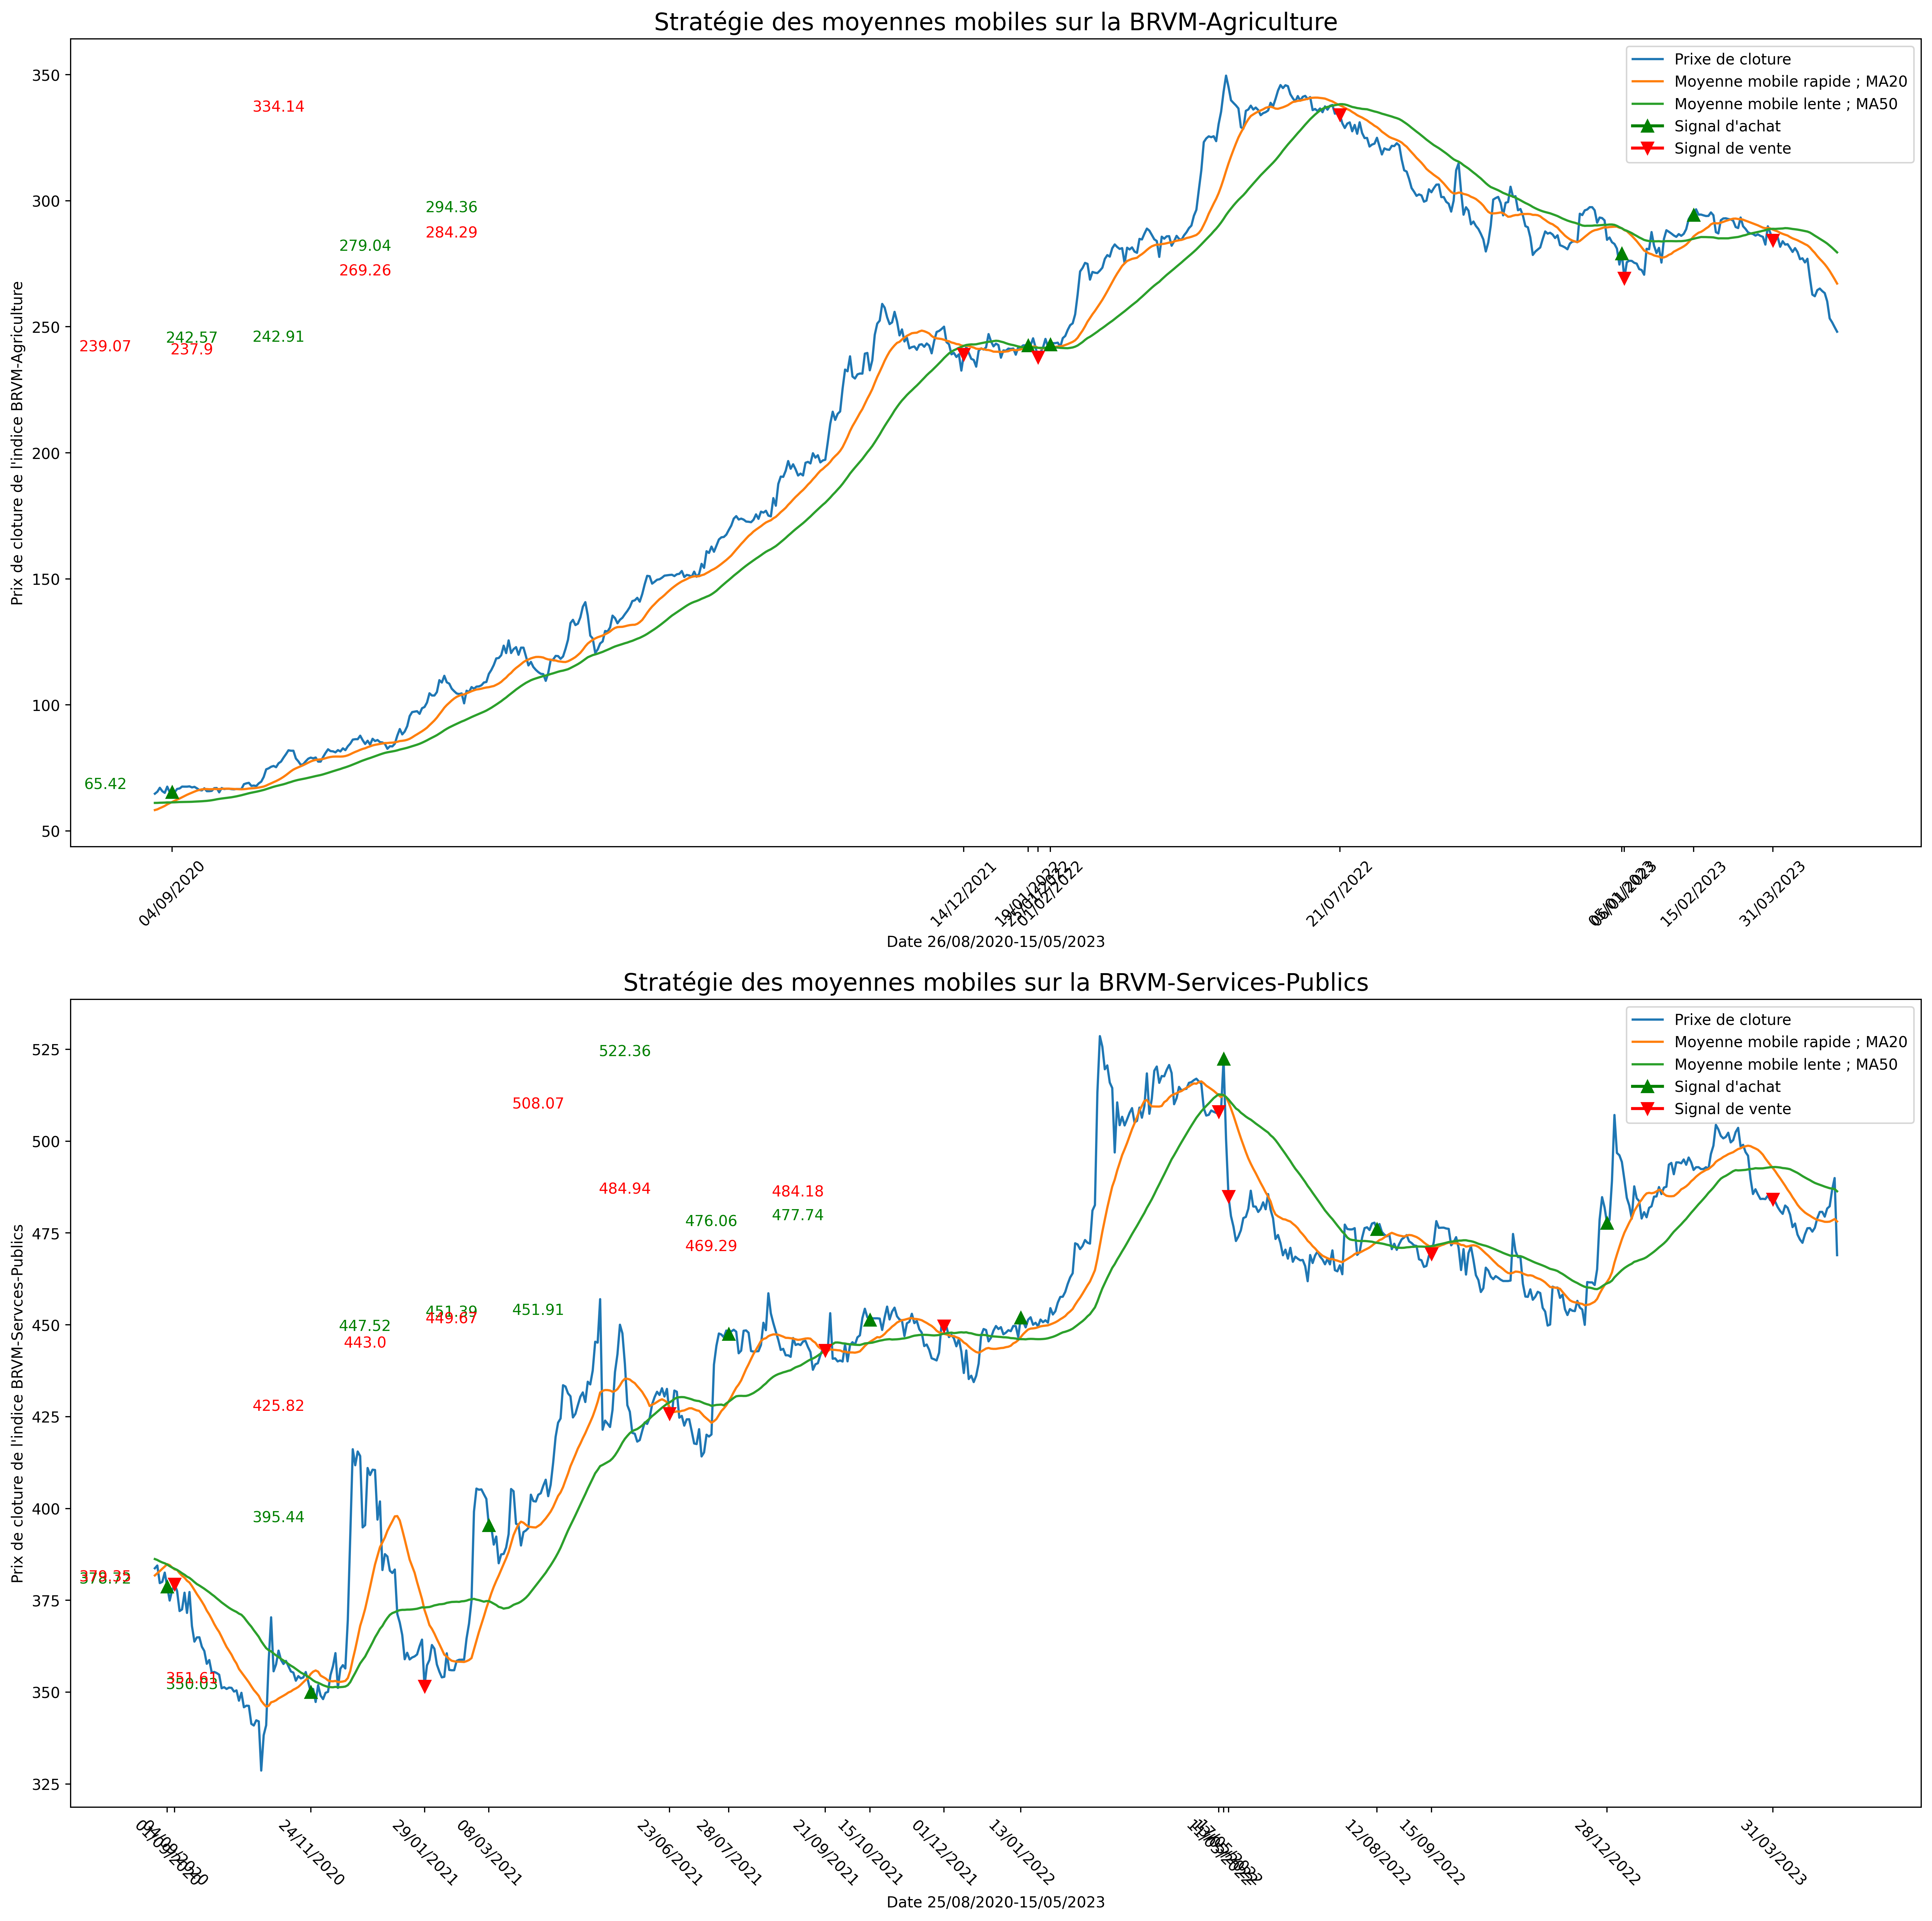
\includegraphics{img/MA-standard.png}
  \caption{Strategie des Moyennes Mobiles avec les périodes
  standard}\label{fig:Strategieux20desux20Moyennesux20Mobilesux20avecux20lesux20puxe9riodesux20standard}
  }
  \end{figure}
\item
  \textbf{Strategie Combine de MACD et de Stochastique avec les périodes
  standard.}\\

  \textbf{"BRVM-Agriculture-BRVM-Services-Publics"}

  \begin{figure}
  \hypertarget{fig:Strategieux20Combineux20deux20MACDux20etux20deux20Stochastiqueux20avecux20lesux20puxe9riodesux20standard}{%
  \centering
  \includegraphics{img/MACD-standard.png}
  \caption{Strategie Combine de MACD et de Stochastique avec les
  périodes
  standard}\label{fig:Strategieux20Combineux20deux20MACDux20etux20deux20Stochastiqueux20avecux20lesux20puxe9riodesux20standard}
  }
  \end{figure}

  La figure 3.3 illustre la stratégie des Moyennes Mobiles sur les
  indices BRVM-Agriculture et BRVM-Services-Publics. L'analyse révèle
  que cette stratégie a généré 10 signaux d'achat et de vente sur
  l'indice BRVM-Agriculture, ainsi qu'un total de 18 signaux d'achat et
  de vente sur l'indice BRVM-Services-Publics. La première transaction
  réalisée sur l'indice BRVM-Agriculture a été la plus bénéfique, car le
  signal d'achat était de 65,42 Fcfa, tandis que le signal de vente
  était de 239,07 Fcfa. Cependant, les deux dernières transactions
  utilisant la stratégie des Moyennes Mobiles se sont soldées par des
  pertes. Ainsi, sur un total de 5 transactions, seules 2 ont été
  enregistrées, soit un taux de réussite de 40 Concernant l'indice
  BRVM-Services-Publics, la stratégie des Moyennes Mobiles a généré un
  total de 18 signaux d'achat et de vente. Parmi ces 18 transactions
  organisées, 14 ont été positives, représentant un taux de réussite de
  77\%. L'analyse des courbes révèle que la 6ème transaction a été la
  plus bénéfique, avec un signal d'achat à un cours de 451,91 Fcfa et un
  signal de vente à un prix de 508,07 Fcfa. De plus, entre le 11, 13 et
  le 17 mai 2022, on peut observer une série de signaux d'achat et de
  vente causée par une chute, un pic, et une rechute des cours entre les
  périodes allant du 10 mai 2022 (où l'indice valait 507,70 Fcfa) au 13
  mai (où l'indice était à 522,36 Fcfa), pour finalement descendre à
  500,63 Fcfa le lendemain. En résumé, la stratégie des Moyennes Mobiles
  a généré un bénéfice total de \textbf{359,46\%} pour l'indice
  BRVM-Agriculture et un bénéfice total de \textbf{11,41\%} pour
  l'indice BRVM-Services-Publics."

  La figure 3.4 illustre la stratégie combinée de l'Oscillateur
  Stochastique et de la moyenne mobile convergence divergence sur les
  indices BRVM-Agriculture et BRVM-Services-Publics. De son analyse, il
  ressort que la méthode combinée de l'Oscillateur Stochastique et de la
  MACD a donné un total de 3 signaux d'achat et de vente. Sur les trois
  signaux obtenus, une seule transaction a été réalisée, soit un signal
  d'achat pour un cours de 311,58 Fcfa et un signal de vente à 294,52
  Fcfa, ce qui représente un faux signal et donc a donné lieu à une
  transaction négative. Par la suite, un signal d'achat a été généré,
  mais malheureusement, dans la suite des données, il n'y a plus eu de
  signal de vente. Au total, la stratégie combinée de l'Oscillateur
  Stochastique et de la moyenne mobile convergence divergence a donné un
  taux de bénéfice de \textbf{-5,48\%} sur la BRVM-Agriculture. En ce
  qui concerne l'indice BRVM-Services-Publics, la stratégie a donné 9
  signaux d'achat et de vente. Nous n'avons pas observé de fausses
  transactions, mais un signal de vente très tôt à la 4ème transaction.
  En somme, la stratégie a donné un bénéfice total de \textbf{29,79\%}
  sur l'indice BRVM-Services-Publics.
\item
  \textbf{Strategie des Moyennes Mobiles (avec les nouveaux
  paramètres).}

  {Maintenant que nous connaissons les périodes qu'il faut, nous allons
  appliquer la stratégie de trading basée sur la moyenne mobile sur les
  indices BRVM-Agriculture et sur les indices BRVM-Services-Publics.}

  \textbf{"BRVM-Agriculture"}

  \begin{figure}
  \hypertarget{fig:Strategieux20desux20Moyennesux20Mobilesux20surux20laux20BRVM-Agri}{%
  \centering
  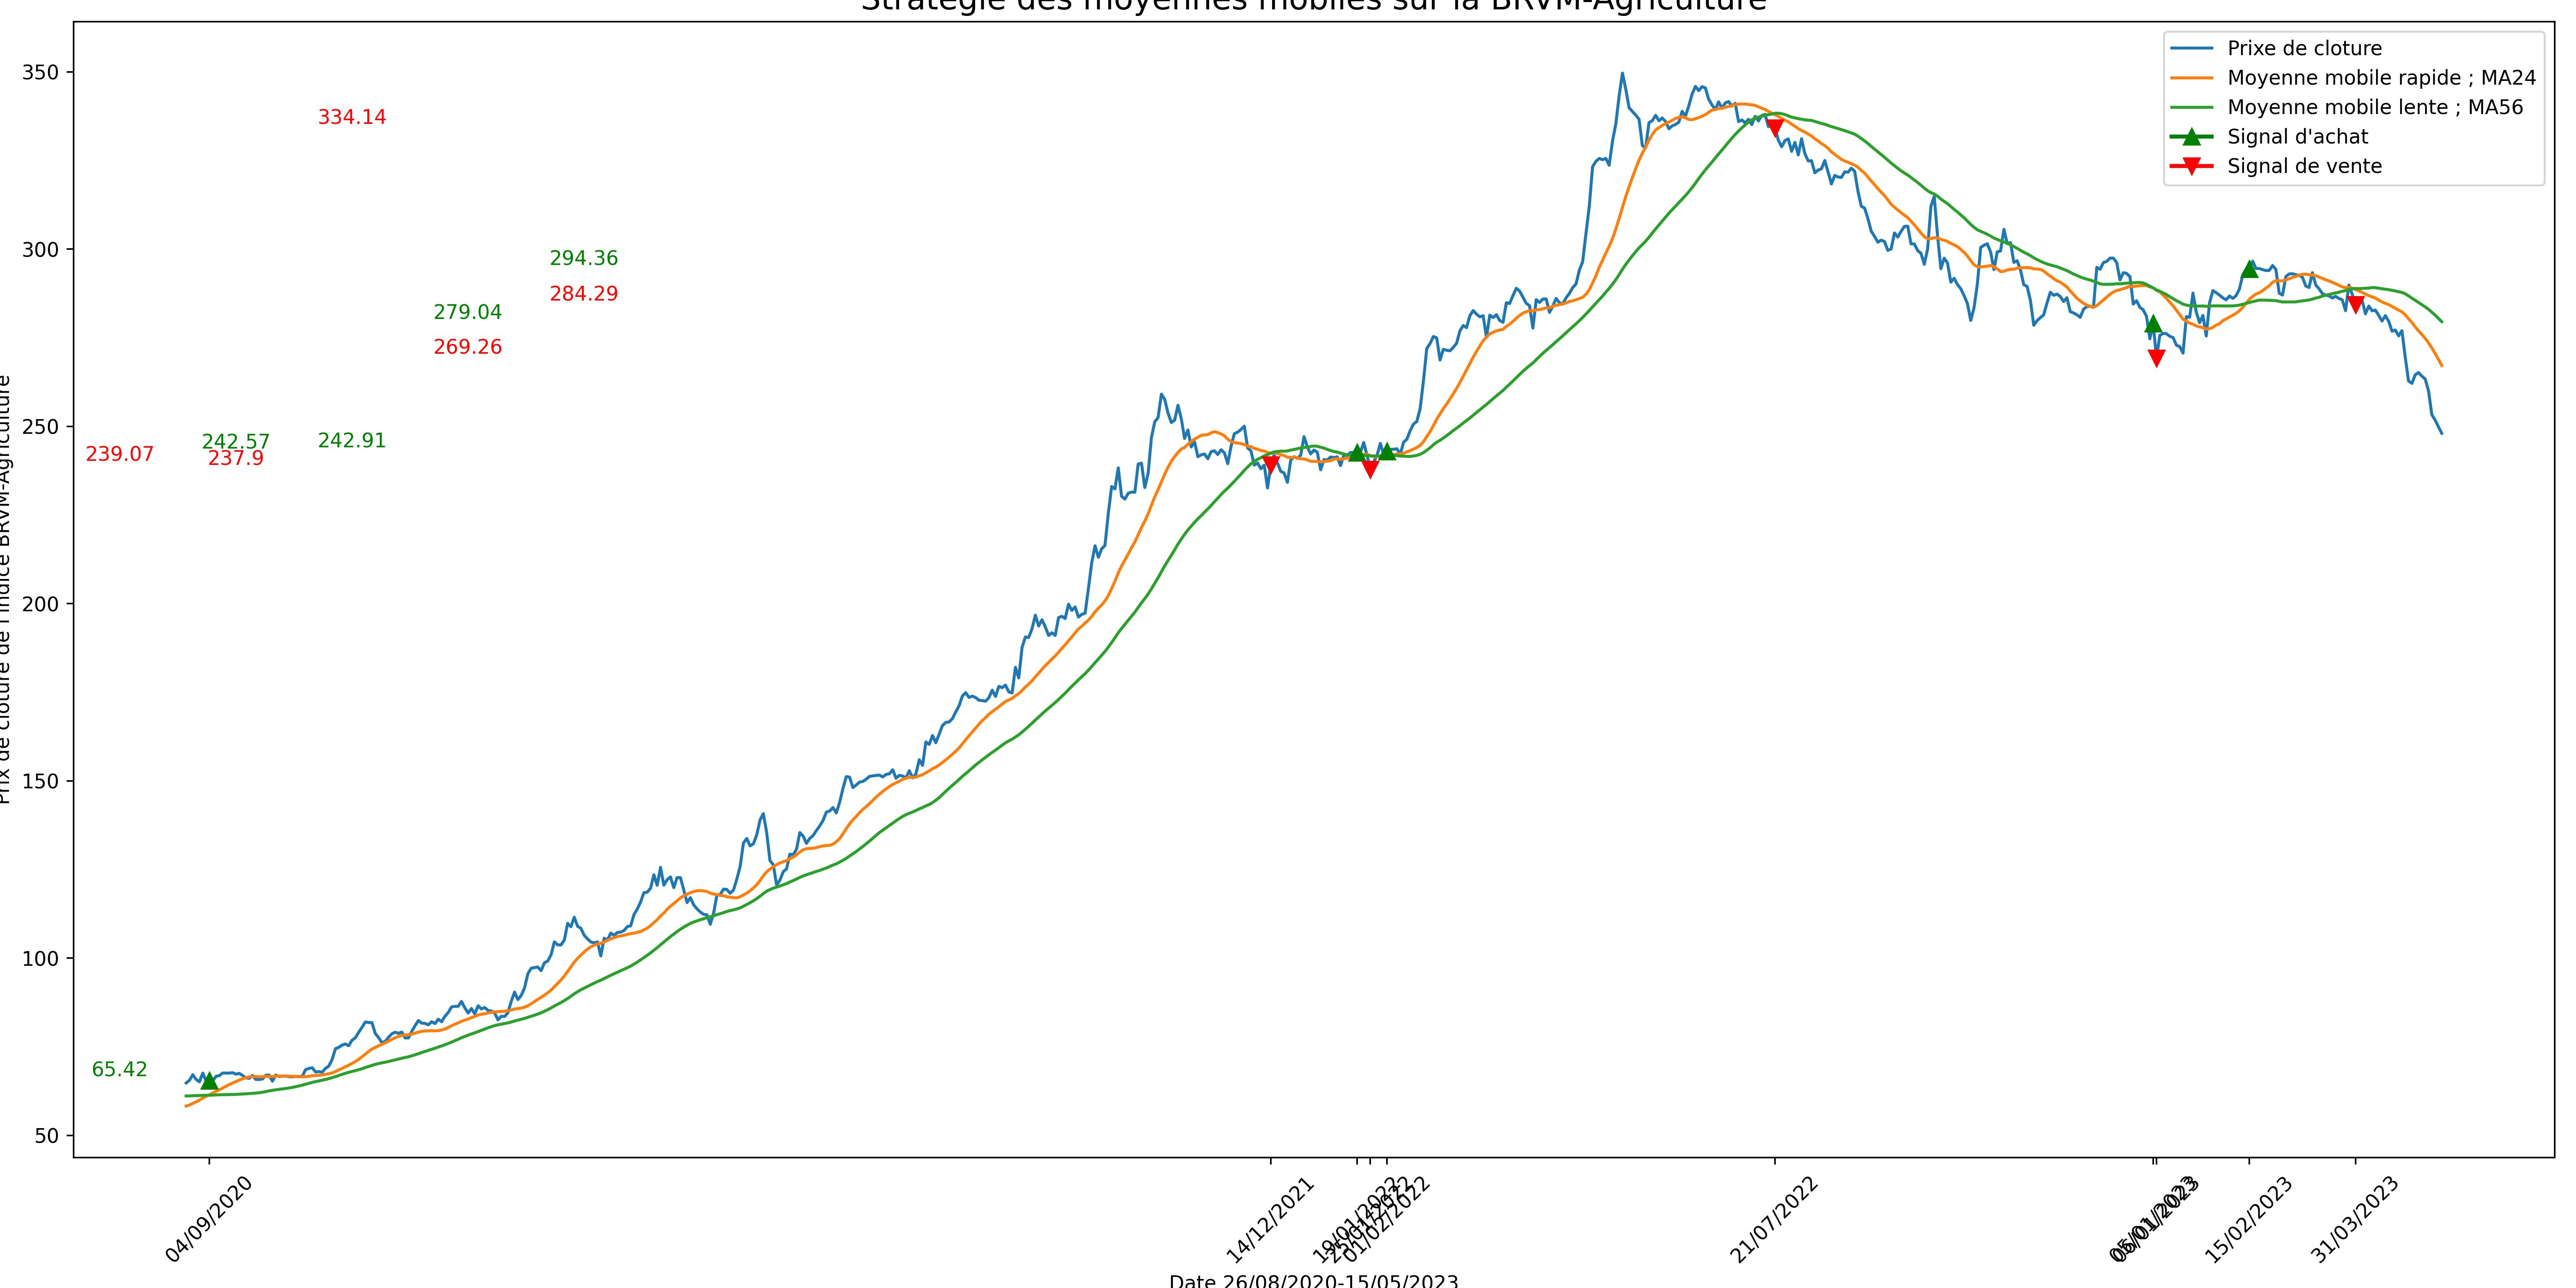
\includegraphics{img/MA-agri.jpg}
  \caption{Strategie des Moyennes Mobiles sur la
  BRVM-Agri}\label{fig:Strategieux20desux20Moyennesux20Mobilesux20surux20laux20BRVM-Agri}
  }
  \end{figure}

  La figure ci-dessus illustre l'application de la stratégie des
  Moyennes Mobiles sur l'indice BRVM-Agriculture. Cette représentation
  graphique présente les tendances de la moyenne mobile arithmétique
  lente et de la moyenne mobile rapide, ainsi que les signaux d'achat et
  de vente. L'analyse de cette figure révèle que la stratégie des
  Moyennes Mobiles a généré un total de 8 signaux d'achat et de vente.

  Sur le graphique de gauche, nous pouvons observer des nombres en rouge
  et en vert. Le nombre en vert représente le prix d'achat de l'actif
  après un signal d'achat, tandis que le nombre en rouge représente le
  prix de vente au signal de vente. Ainsi, si le nombre en rouge est
  inférieur au nombre en vert, cela signifie que la transaction a
  entraîné une perte.

  Dans la figure ci-dessous, nous pouvons remarquer que toutes les
  transactions sont positives, indiquant l'absence de faux signaux, ou
  presque. Toutefois, entre le 26 janvier 2022 et le 2 février 2022,
  nous avons observé deux signaux d'achat et de vente très rapprochés en
  raison d'une fluctuation inhabituelle du cours de l'indice. Malgré
  cela, les transactions ont été un succès car le prix d'achat était de
  236,96 et le prix de vente de 242,91." La méthode des Moyennes Mobiles
  sur la BRVM-Agriculture à donner \textbf{367,167\%}

  \textbf{"BRVM-Services-Publics"}

  \begin{figure}
  \hypertarget{fig:Strategieux20desux20Moyennesux20Mobilesux20surux20laux20BRVM-Services-Publics}{%
  \centering
  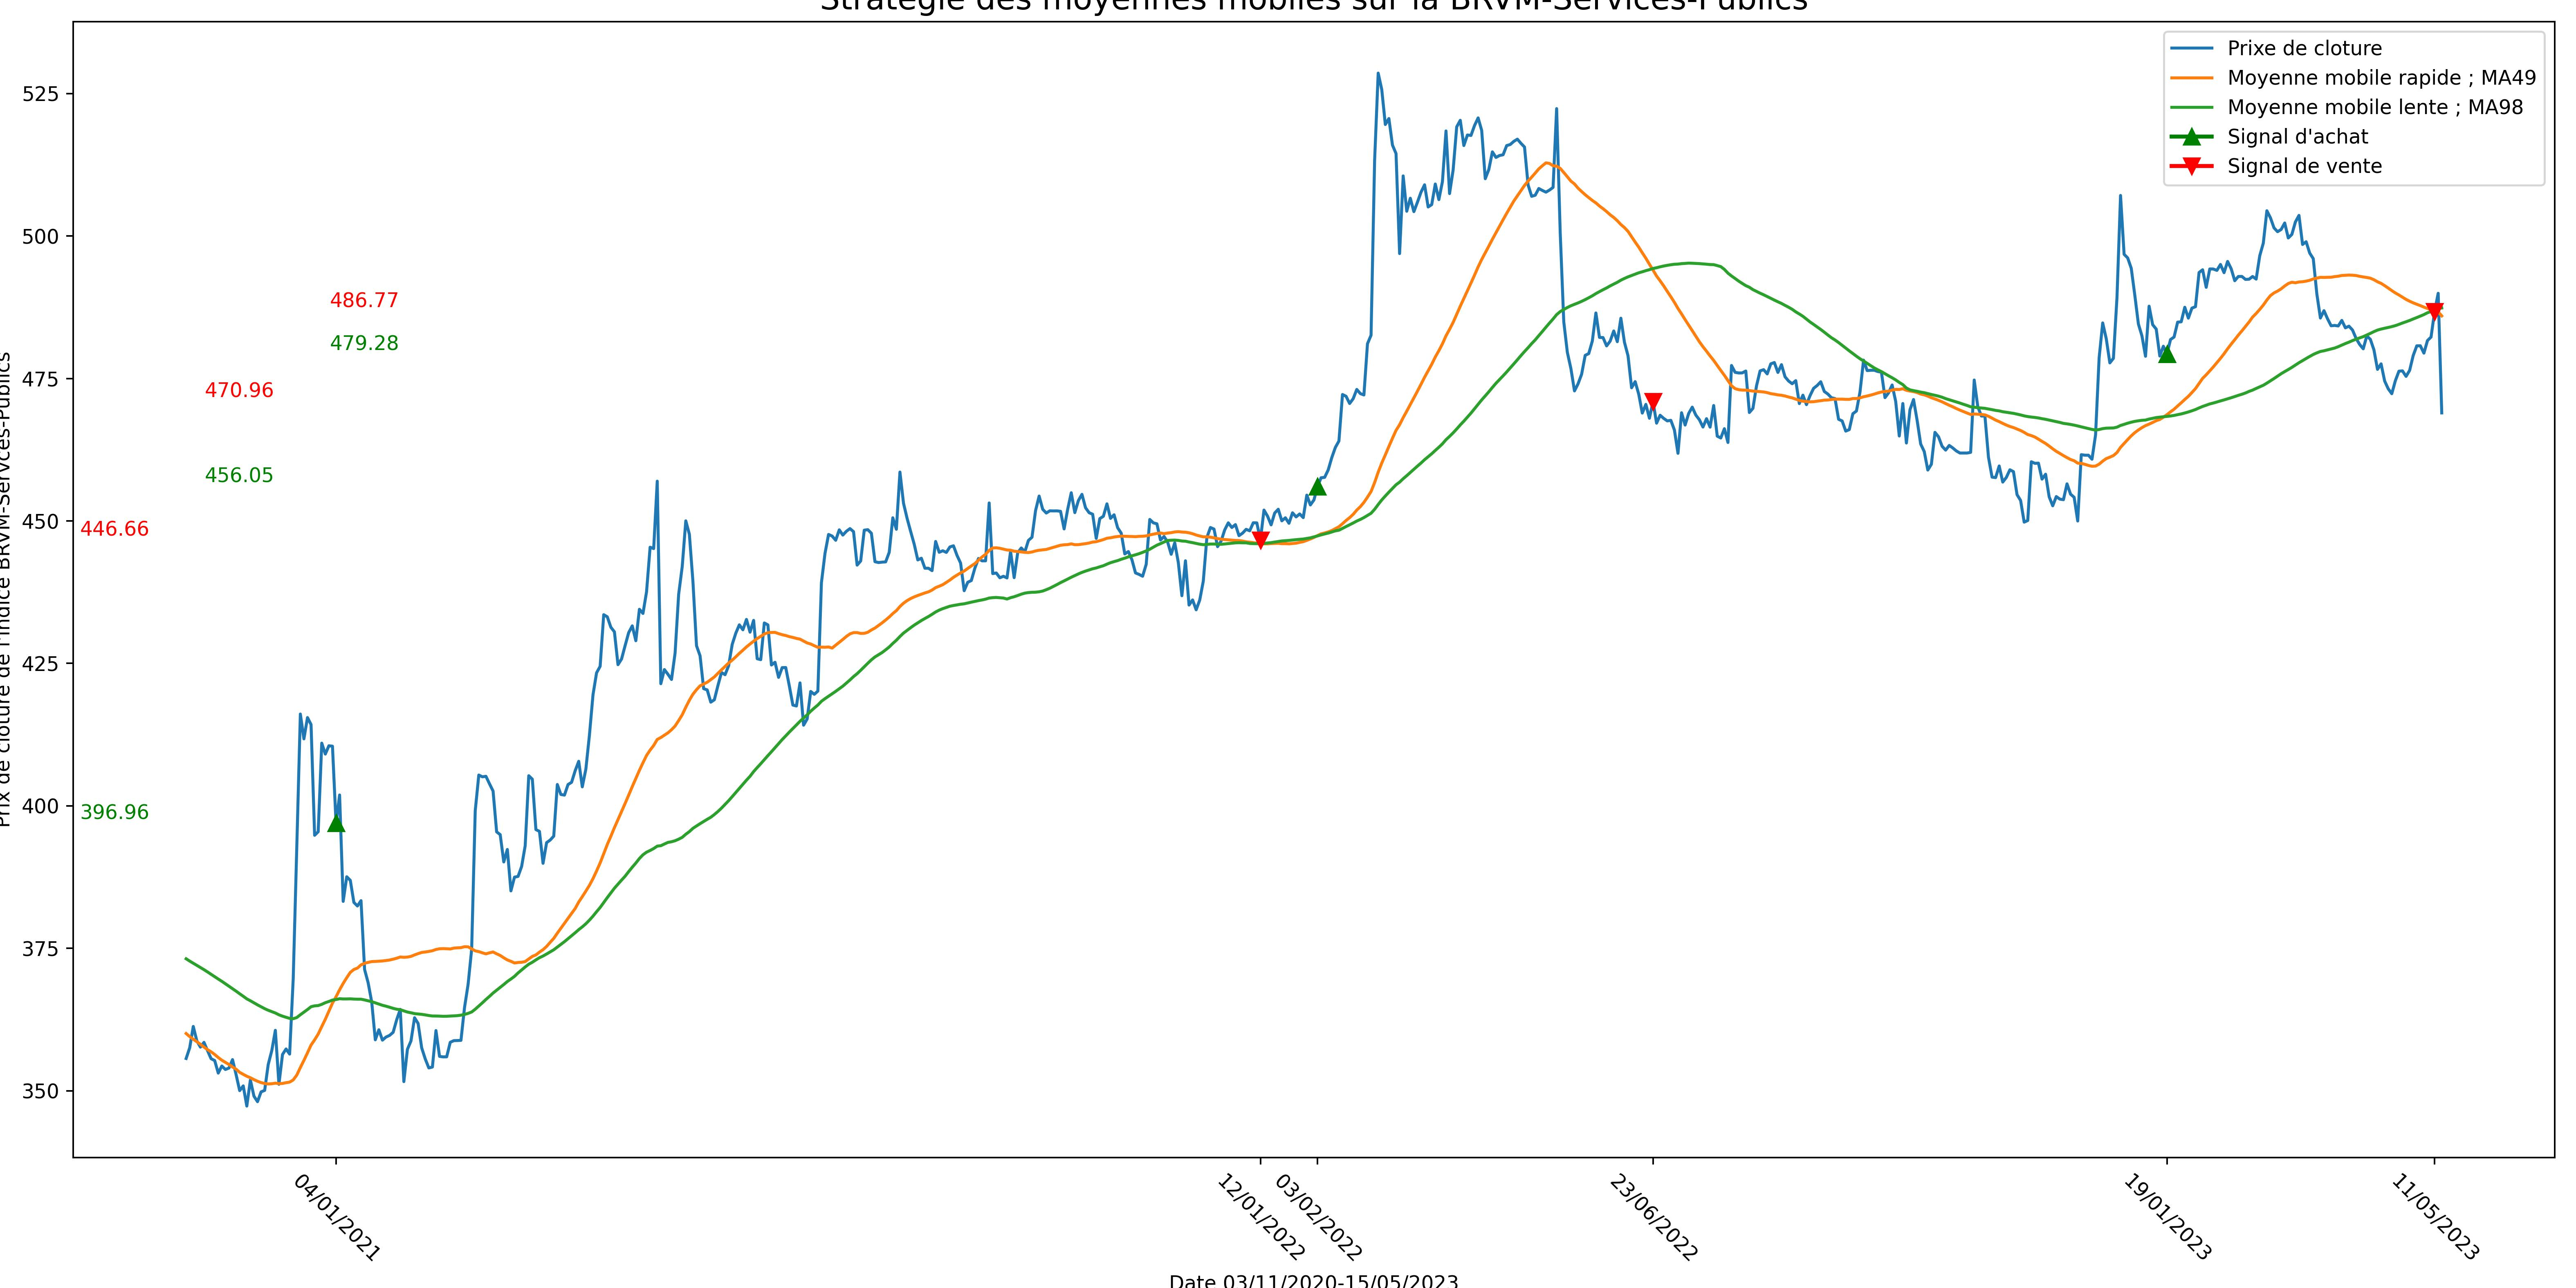
\includegraphics{img/MA-public.jpg}
  \caption{Strategie des Moyennes Mobiles sur la
  BRVM-Services-Publics}\label{fig:Strategieux20desux20Moyennesux20Mobilesux20surux20laux20BRVM-Services-Publics}
  }
  \end{figure}

  La représentation graphique ci-dessus offre une vue de la stratégie de
  trading des Moyennes Mobiles sur l'indice BRVM-Services-Publics. Dans
  le coin à droite ce trouve des informations sur ce que représente
  chaque courbe. Ainsi nous pouvons lire que la courbe en vert
  représente la moyenne mobile sur 98 jours ('lente') et celle orange la
  moyenne mobile sur 48 jours ('rapide'). De son analyse il ressort
  qu'un total de trois transactions on été effectuées dont la plus
  bénéfique est la première transaction. En effet lors de cette
  transaction l'indice à été acheter au prix de 396,96 Fcfa et revendu à
  446,66 Fcfa.

  Remarquons cependant que le signal d'achat est un signal légèrement en
  retard car il survient après un pique observer entre le 09 décembre
  2020 et le 17 décembre 2020 ou le cours de l'indice est passe de
  351,14 fcfa à 416,12 Fcfa. Il aurait été donc plus bénéfique que le
  signal d'achat ait été générer un peux plus tôt. Mais cela est dur à
  ce mouvement inhabituelle observer durant cette période de temps. Le
  phénomène contraire s'observe également au niveau de la deuxième
  transaction ou le signal de vente est venu un peu trop tardivement
  après un que l'indice est atteint son plus grand pique. En somme la
  Stratégie des Moyennes Mobiles sur l'indice BRVM-Services-Publics à
  engendrer un bénéfice total de \textbf{18,01 \%}
\item
  \textbf{Strategie Combiné de l'Oscillateur Stochatique et de la
  Moyenne Mobile Convergence Divergence (avec les nouveaux paramètres).}

  \textbf{"BRVM-Agriculture"}

  \begin{figure}
  \hypertarget{fig:Strategieux20Combineux20deux20MACDux20etux20deux20Stochastiqueux20surux20lux27indiceux20Agriculture}{%
  \centering
  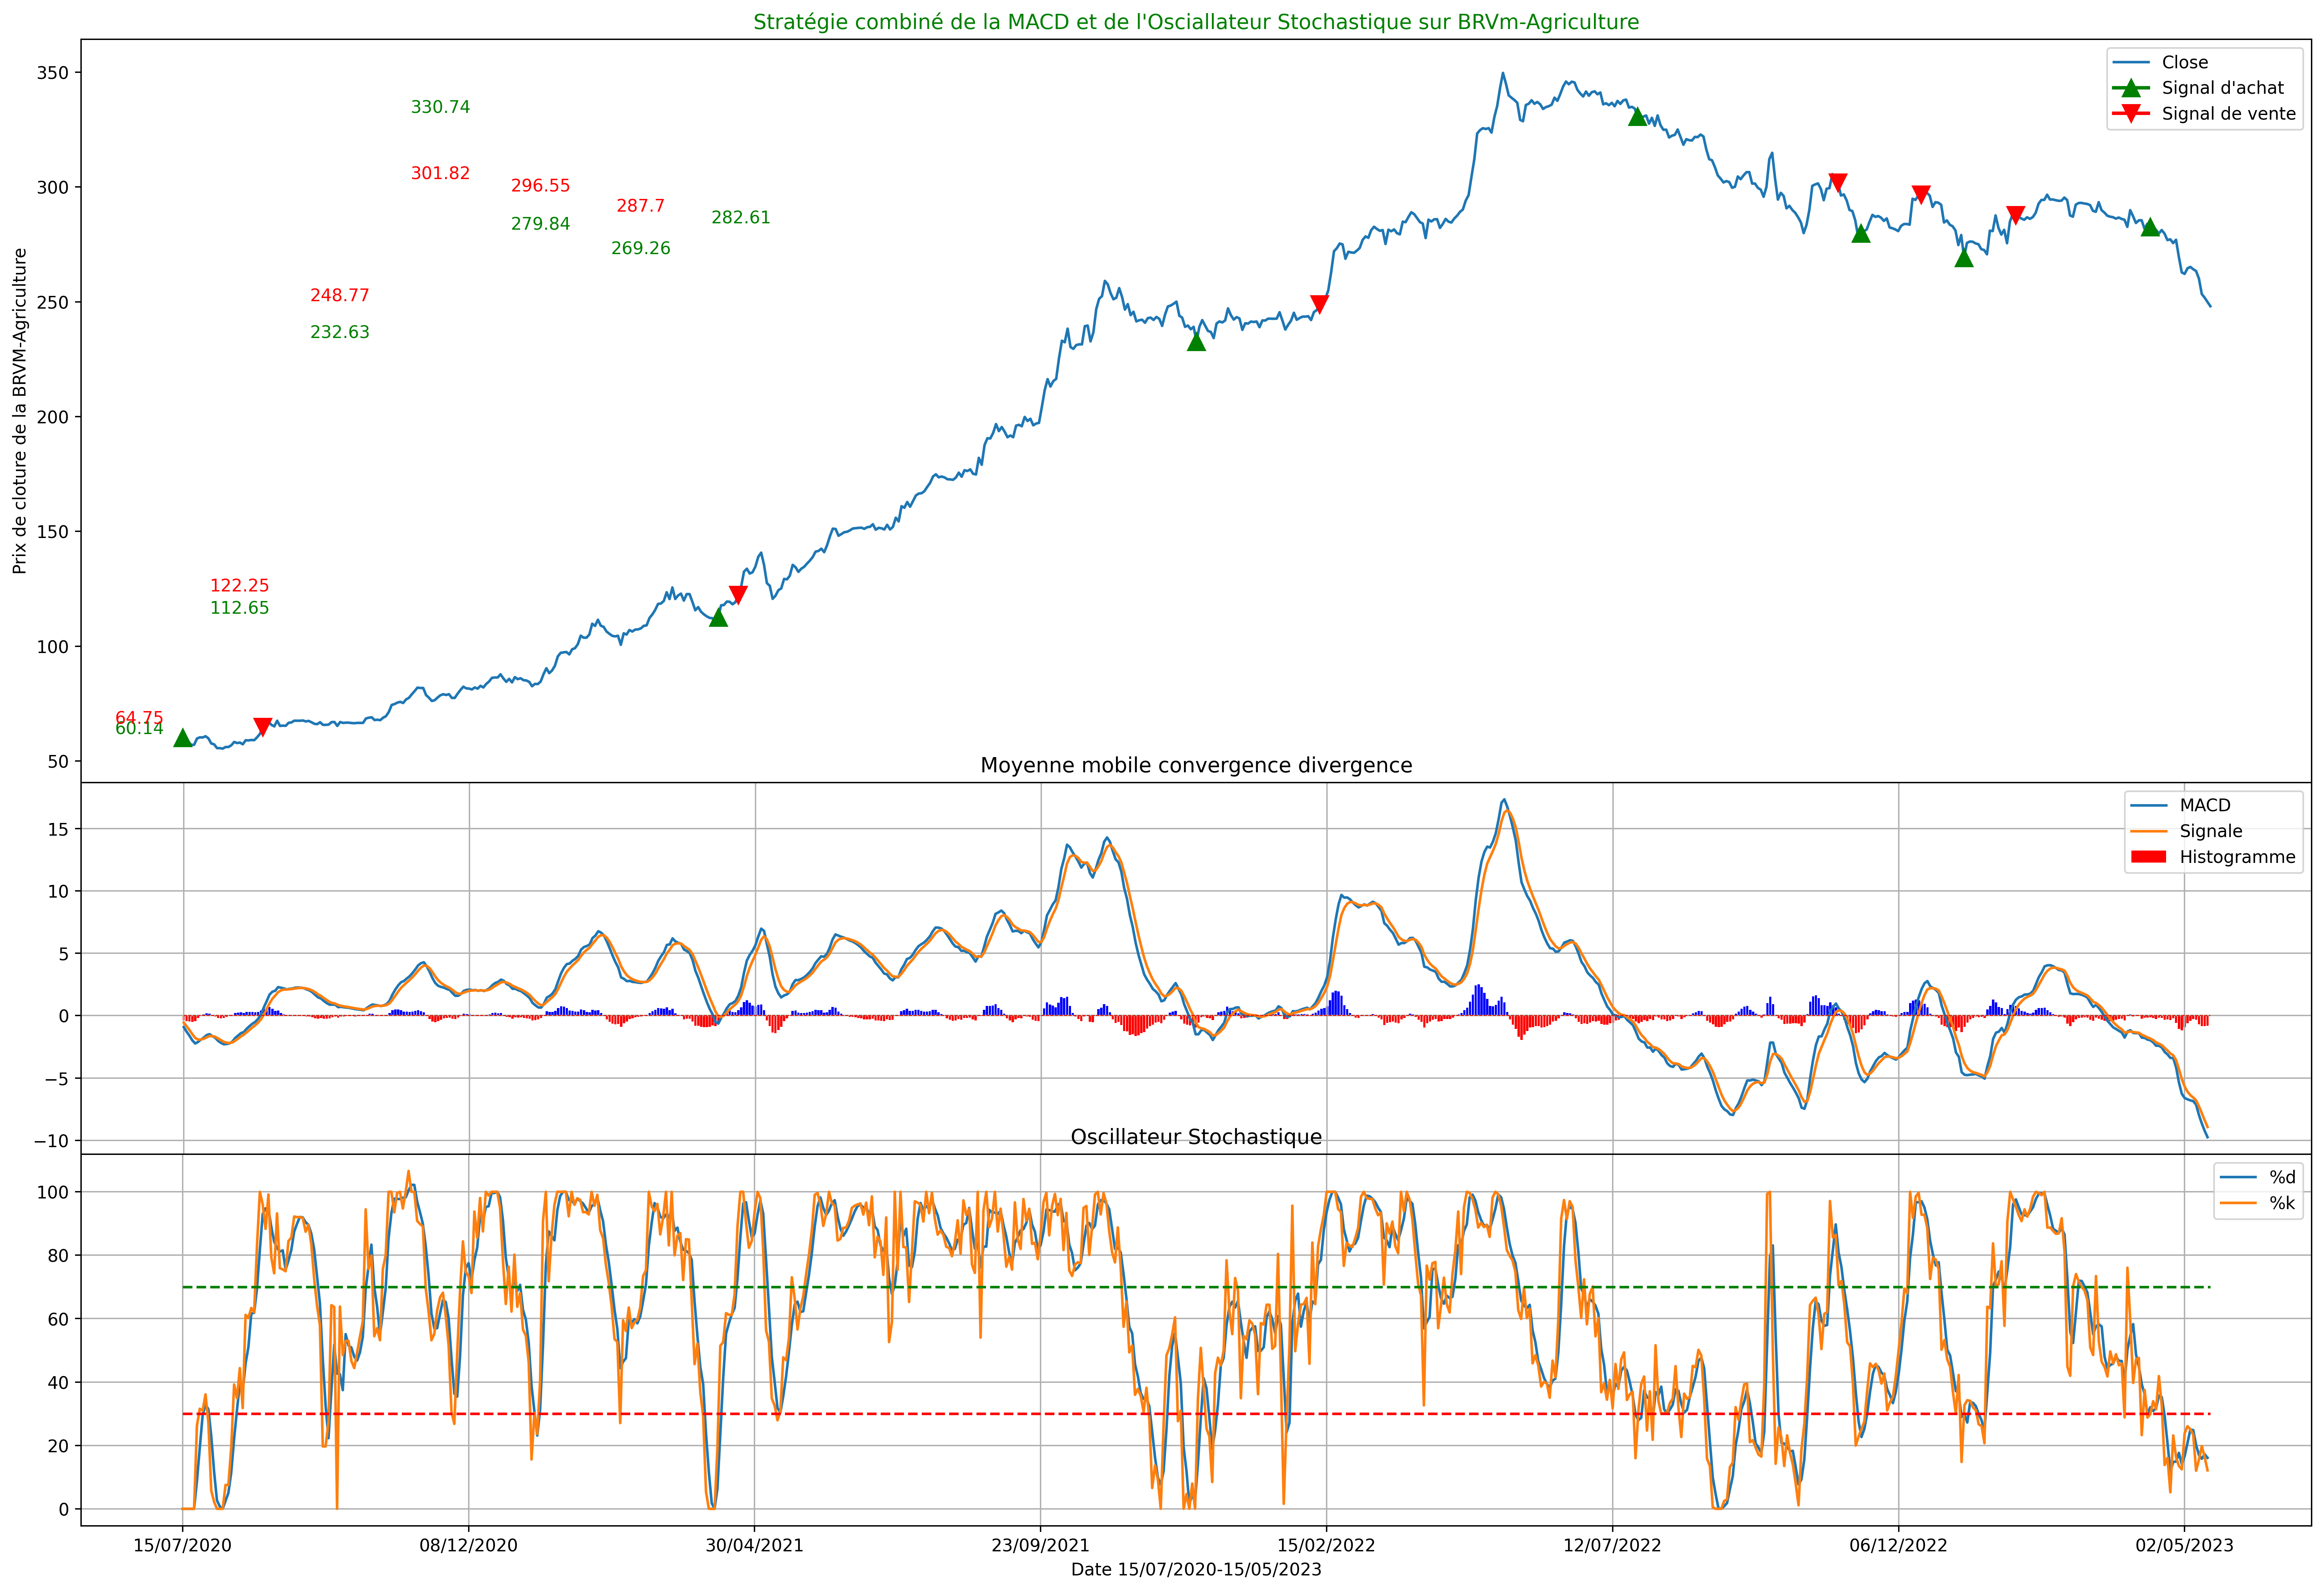
\includegraphics{img/MACD-Agri.png}
  \caption{Strategie Combine de MACD et de Stochastique sur l'indice
  Agriculture}\label{fig:Strategieux20Combineux20deux20MACDux20etux20deux20Stochastiqueux20surux20lux27indiceux20Agriculture}
  }
  \end{figure}

  {La représentation graphique ci-dessus, illustre la courbe du cours de
  l'indice BRVM-Agriculture , la Moyenne Mobile Convergence Divergence ,
  ainsi que l'Oscillateur Stochastique. De cette représentation
  graphique, nous pouvons observer que les courbes de l'Oscillateur
  Stochastique dépasse très fréquemment la barre des 70\% ce qui indique
  à chaque fois que le marché est dans un état de surachat ce qui
  représente un signal de vente. Cependant afin de valider ce signal il
  faut que la MACD soit supérieur à zéro. De plus on peut remarquer que
  après le 12 juillet 2022 une fluctuation inhabituelle des cours de
  l'indice, ce qui a générer un faux signal de vente et qui donc a
  conduit une perte au cours de cette transaction. Suivant les cours des
  transactions en haut à gauche (du côté de la courbe des cours de
  l'indice) nous pouvons observer que le prix d'achat de la valeur à
  cette transaction était de 330,74 Fcfa et son prix de vente de 301,81
  Fcfa. Finalement la stratégie combinée de l'Oscillateur Stochastique
  et de la Moyenne Mobile Convergence Divergence à donner un bénéfice
  total de \textbf{29,105\%} }

  \textbf{"BRVM-Services-Publics"}

  \begin{figure}
  \hypertarget{fig:Strategieux20desux20Moyennesux20Mobilesux20surux20laux20BRVM-Services-Publics}{%
  \centering
  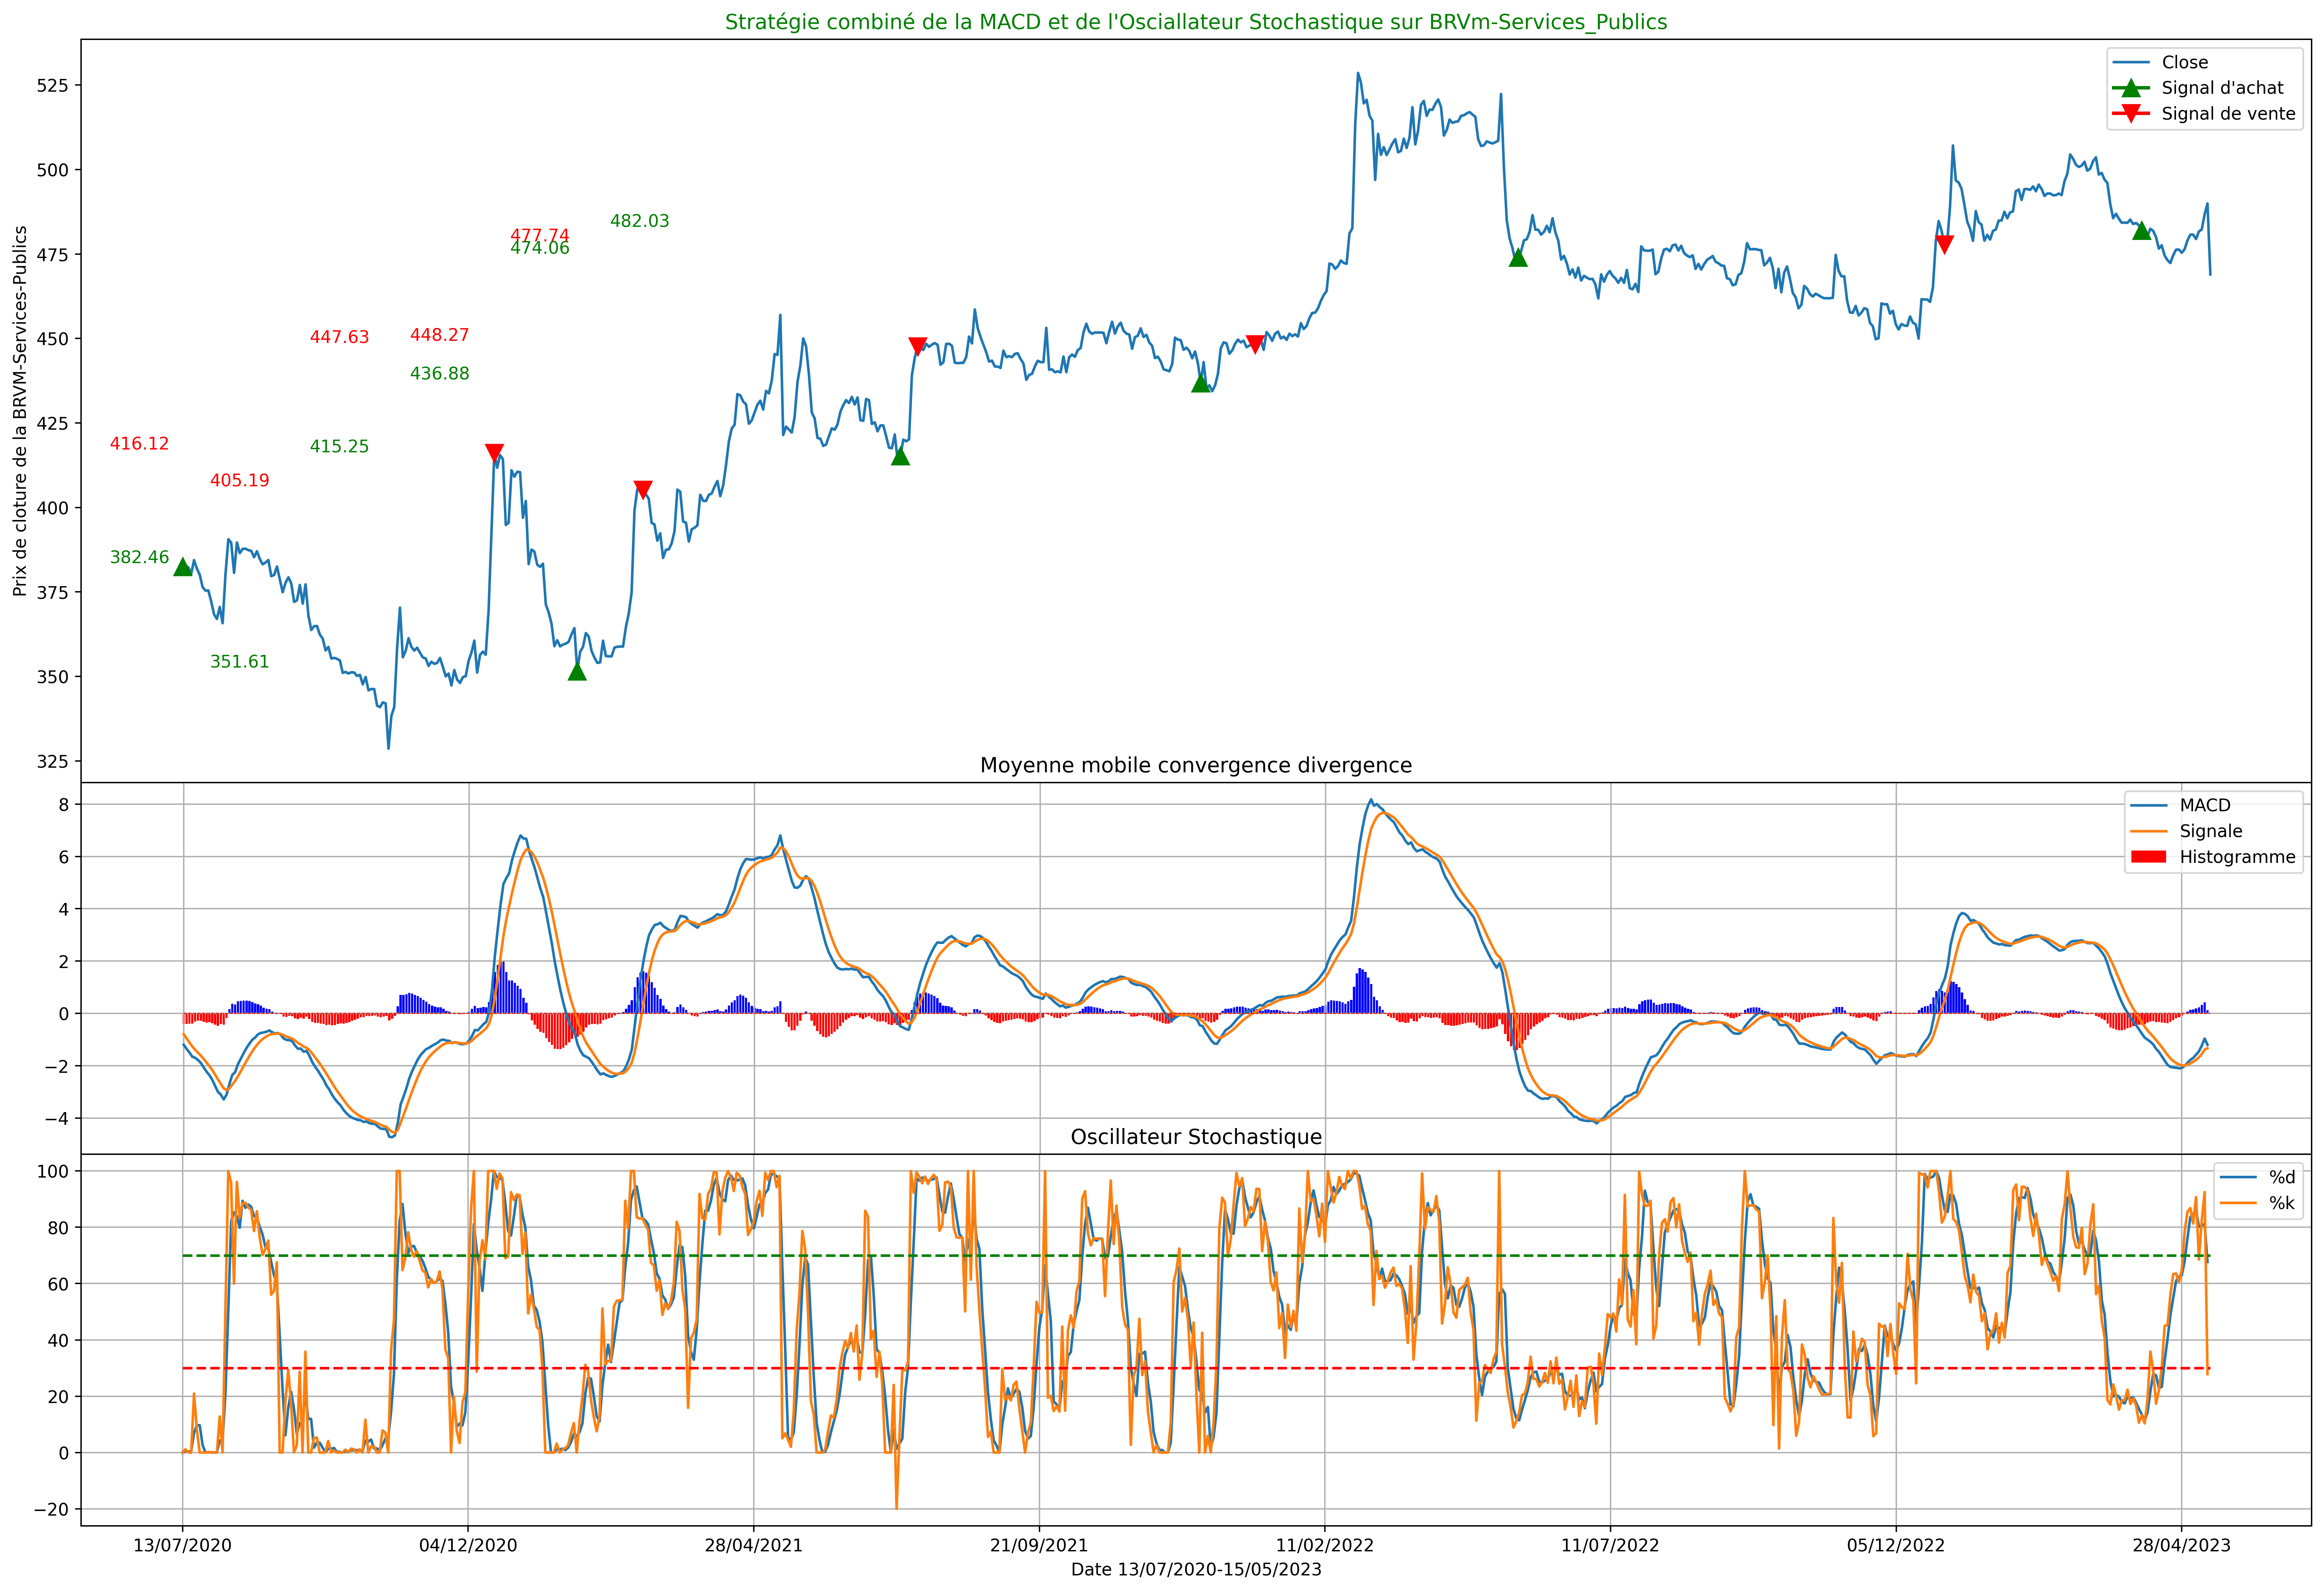
\includegraphics{img/MACD-Public.png}
  \caption{Strategie des Moyennes Mobiles sur la
  BRVM-Services-Publics}\label{fig:Strategieux20desux20Moyennesux20Mobilesux20surux20laux20BRVM-Services-Publics}
  }
  \end{figure}

  La figure ci-dessus présente l'application de la stratégie combinée de
  l'oscillateur Stochastique et de la Moyenne Mobile Convergence
  Divergence sur l'indice BRVM-Service-Publics. De son analyse il
  ressort qu'il y a une répartition équitable des signaux d'achat et de
  vente générer par la Moyenne Mobile Convergence Divergence. En tout
  nous avons obtenu 9 signaux d'achat et de vente dont un signal d'achat
  final. La transaction la plus bénéfique réalisé est la deuxième ou le
  prix d'achat de la valeur était de 351,61 Fcfa et son prix de vente de
  405,19 Fcfa. Notons que toutes les transactions sont positives et que
  le taux de bénéfice total réalisé à la fin de l'application de la
  stratégie est de \textbf{39,758\&}.

  Bien que toute les transaction soit positive on observe que le 5eme
  signal de vente est venu un peut trop tôt car dans la suite de
  l'évolution des cours, le prix de l'indice à dépasser les 500 Fcfa
  contre un signal d'achat ou l'indice coutait 474,06 Fcfa. Ce retard
  est d'autant plus remarquable au niveau de la 4eme transaction où le
  signal de vente est venu vraiment très tôt cas juste après le signal
  de vente l'indice à atteint sont cours maximal de \textbf{528,59
  Fcfa}.

  \subsubsection{Interprétation des résultats et vérifications des
  hypothèses.}\label{interpruxe9tation-des-ruxe9sultats-et-vuxe9rifications-des-hypothuxe8ses.}

  D'après les analyses, la stratégie des Moyennes Mobile sur l'indice
  BRVM-Agriculture à générer au total de 8 signaux d'achat et de vente
  et 6 signaux d'achat et de vente sur l'indice BRVM-Services-Publics.
  En ce qui concerne la stratégie combinée de l'Oscillateur Stochastique
  et de la Moyenne Mobile Convergence Divergence, elle à donner 13
  signaux d'achat et de vente pour l'indice BRVM-Agriculture et 11
  signaux d'achat et de vente pour l'indice BRVM-Services-Publics, ce
  qui fait un total de 24 signaux. Nous remarquons donc que nombre total
  de signaux obtenu grâce à la stratégie des Moyennes Mobiles ainsi que
  le nombre total de signaux individuel pour chaque indice est inférieur
  aux signaux obtenu grâce à la stratégie combiné de l'oscillateur
  stochastique et de la Moyenne Mobile Convergence Divergence. Alors
  l'hypothèses selon laquelle la méthode des Moyennes Mobiles génère
  plus de signal d'achat et de ventes que la méthodes combinée de
  l'Oscillateur Stochastique et de la des Moyennes Mobiles convergence
  divergence n'est pas vérifier.

  De plus il ressort que l'application de la stratégie des moyennes
  mobile à générer un bénéfice total de 367,167\% sur l'indice
  BRVM-Agriculture et un total de 18,01\% sur l'indice
  BRVM-Services-Publics. Par ailleurs la stratégie combinée de
  l'Oscillateur Stochastique et de la Moyenne Mobile Convergence
  Divergence quand à elle a donné un bénéfice total de 29,105\% sur
  l'indice BRVM-Agriculture contre un bénéfice total de 39,758\% pour
  l'indice BRVM-Service-Publics. Il ressort de ces résultats que
  \textbf{la stratégie des Moyennes Mobile donne plus de bénéfice sur
  l'indice BRVM-Agriculture que sur l'indice BRVM-Services-Publics.
  Alors que la stratégie Combiné de l'Oscillateur Stochastique et de la
  Moyenne Mobile Convergence Divergence donne plus de bénéfices sur
  l'indice BRVM-Service-Public que sur l'indice BRVM-Agriculture}. En
  somme la stratégie des Moyennes Mobiles donne un total de 385,177\%
  pour les deux indices et la méthode combinée de l'Oscillateur
  Stochastique et de la Moyenne Mobile Convergence Divergence produit un
  total de 68,863\% pour les deux indices. Alors l'hypothèses selon
  laquelle la méthode combinée de l'Oscillateur Stochastique et de la
  Moyenne Mobile Convergence Divergence génère plus de bénéfices que la
  méthode des Moyennes Mobile n'est pas vérifié.

  \subsection{Approche de solution}\label{approche-de-solution}

  { Afin d'optimiser au mieux le profil des investisseurs à la Bourse
  Régional des valeurs Mobilière, notamment ceux qui investissent dans
  le domaine des Services Publics et de l'Agriculture, entre la
  stratégie de la moyenne mobile et de la méthode Combiné de
  l'Oscillateur Stochastique et de la Moyenne Mobile Convergence
  Divergence au vu des résultats obtenus dans cet études nous
  recommandons vivement l'utilisation de la stratégie des Moyennes
  Mobile sur l'indice BRVM-Agriculture et l'usage de la méthode Combiné
  de l'Oscillateur stochastique et de la Moyenne Mobile Convergence
  Divergence sur l'indice BRVM-Services-Publics. De plus dans le cadre
  de l'application de ces stratégies nous recommandons de faire des
  simulations afin de déterminer les paramètres pour la stratégie des
  moyennes mobiles qui permettent d'obtenir de meilleur bénéfice pour
  les tendance futur du marché et l'usage de nos critère de validations
  des paramètres élaborer dans le cadre de cette étude comparative. }
\end{itemize}

\section*{Conclusion}\label{conclusion}
\addcontentsline{toc}{section}{Conclusion}

{La stratégie des moyennes mobile et celle de la Moyenne mobile
Convergence Divergence se base sur l'indicateur de tendance de moyenne
mobile, et la Stratégie de l'Oscillateur se base sur l'indicateur de de
Momentum. Le but de cette étude était de déterminer la stratégie la plus
performante entre ces deux méthodes pour les indices BRVM-Agriculture et
BRVM-Services-Publics. Apres l'analyse des résultats, il est clair que
la méthode des moyennes mobile performe le plus sur l'indice
BRVM-Agriculture et la méthode combinée de l'Oscillateur Stochastique et
de la Moyenne Mobile Convergence performe la mieux pour l'indice
BRVM-Services-Publics. Notre étude met l'accent sur les différentes
paramètres des stratégies de trading, notamment les périodes des
moyennes mobile. Bien que l'objectif de cette étude était était de
comparer les stratégies de trading sur les indices BRVM-Agriculture et
BRVM-Services-Publics, il a été élaborer des critères permettant de
valider les paramètre d'une Stratégie spécifique. Ainsi donc pour un
investisseurs voulant bénéficier des résultats de ce travail il serait
préférable de reprendre les analyse affecter dans cette étude tout en
suivant toute les étapes élaborer pour bien choisir la stratégie la plus
performante pour son actif financier. }

{13}\\
\url{https://genevatradecenter.com/analyser-interpreter-une-tendance-trading/#:%7E:text=Il%20existe%20trois%20principaux%20types,terme%20et%20%C3%A0%20long%20terme}\strut \\
27/07/2023 - 10h

\hfill\break
\url{https://economy-pedia.com/11037482-investor-profile}\\
27/07/2023 - 15h

\emph{ZIAD SROUGI Avril 1993 : Analyse technique du taux de change
nominal \textbar{} UNIVERSITE DE MONTREAL \textbar{} Département de
sciences économiques faculté des arts et des sciences.}

\hfill\break
\url{https://www.avatrade.fr/education/technical-analysis-indicators-strategies/support-and-resistance}\\
26/07/2023 - 22h

\hfill\break
\url{https://www.forexagone.com/blog/2122-les-trois-types-de-tendance-en-analyse-graphique}\\
27/07/2023 - 03h

\emph{Tendance baissière-Qu'est ce que c'est, définition et conceps :}\\
\url{https://economy-pedia.com/11032621-downtrend}

\emph{Les 3 Objectifs de trading \textbar{} Maxime PARRA \textbar{} 23
novembre 2018}\\
\url{https://www.newtrading.fr/objectifs-trading#:%7E:text=Dans%20quel%20but%20acheter%20et,G%C3%A9rer%2C%20Prot%C3%A9ger%2C%20ou%20Sp%C3%A9culer.}\strut \\
31/07/2023

\emph{Time Horizon}\\
\url{https://frfbs.com/glossary/time-horizon-36%20}

\emph{Actif financier}\\
\url{https://www.lafinancepourtous.com/outils/dictionnaire/actif-financier/}

\emph{Volatilité}\\
\url{https://www.lafinancepourtous.com/decryptages/marches-financiers/fonctionnement-du-marche/volatilite/#:%7E:text=La%20volatilit%C3%A9%20d'un%20titre,cours%20des%20march%C3%A9s%20sont%20instables.}

\emph{Action}\\
\url{https://www.ig.com/fr/glossaire-trading/Cours-de-l-action-definition#:%7E:text=Le%20cours%20d'une%20action%20correspond%20au%20montant%20n%C3%A9cessaire%20pour,ne%20r%C3%A9pond%20pas%20aux%20attentes.}
